\documentclass [11pt,twoside]{article}
\usepackage[utf8]{inputenc}
\usepackage[T1]{fontenc}

%Page margins, header and footer positions
\usepackage{geometry}
 \geometry{
 a4paper,
 total={210mm,297mm},
 left=25mm,
 right=25mm,
 top=30mm,
 bottom=25mm,
 headsep=7mm}

\interfootnotelinepenalty=10000

%To display filling dots in the TOC for all entries
\usepackage[titles]{tocloft}
\renewcommand{\cftsecleader}{\cftdotfill{\cftdotsep}}

%Define new header and footer style
\usepackage{fancyhdr}

\pagestyle{fancy}
\fancyhf{}
\lhead{\color{Gray}{\small{Travlendar+ project by YOUR NAMES}}}
\lfoot{\textcolor{Gray}{\small{Copyright © 2017, YOUR NAMES – All rights reserved}}}
\rfoot{\textcolor{Gray}{\thepage}}
\renewcommand{\headrulewidth}{0pt}

%PACKAGES
\usepackage{wasysym}
\usepackage{pifont}

\newcommand{\supported}{\ding{52}\xspace}
\newcommand{\unsupported}{\ding{55}\xspace}
\newcommand{\partsupported}{\textcolor{black!40}{\ding{52}}\xspace}
\newcommand{\lowsupported}{\textcolor{black!20}{\ding{52}}\xspace}
\newcommand{\unknowsupported}{\textbf{?}\xspace}

%Font: Times
\usepackage{times}
%Change monospaced font
\renewcommand{\ttdefault}{lmtt}

%tables
\usepackage{tabu}
\usepackage{tabularx}
\usepackage{ltablex}
\usepackage{longtable}
\usepackage{float} % To allow the use of H modifier in long tables

%landscape mode
\usepackage{pdflscape}
\usepackage{rotating}
\usepackage{caption}

%make landscape mode be sensitive to even and odd pages
%start
\def\myrotate{\ifodd\c@page\else-\fi 90}
\makeatletter
\global\let\orig@begin@landscape=\landscape%
\global\let\orig@end@landscape=\endlandscape%
\gdef\@true{1}
\gdef\@false{0}
\gdef\landscape{%
    \global\let\within@landscape=\@true%
    \orig@begin@landscape%
}%
\gdef\endlandscape{%
    \orig@end@landscape%
    \global\let\within@landscape=\@false%
}%
\@ifpackageloaded{pdflscape}{%
    \gdef\pdf@landscape@rotate{\PLS@Rotate}%
}{
    \gdef\pdf@landscape@rotate#1{}%
}
\let\latex@outputpage\@outputpage
\def\@outputpage{
    \ifx\within@landscape\@true%
        \if@twoside%
            \ifodd\c@page%
                \gdef\LS@rot{\setbox\@outputbox\vbox{%
                    \pdf@landscape@rotate{-90}%
                    \hbox{\rotatebox{90}{\hbox{\rotatebox{180}{\box\@outputbox}}}}}%
                }%
            \else%
                \gdef\LS@rot{\setbox\@outputbox\vbox{%
                    \pdf@landscape@rotate{+90}%
                    \hbox{\rotatebox{90}{\hbox{\rotatebox{0}{\box\@outputbox}}}}}%
                }%
            \fi%
        \else%
            \gdef\LS@rot{\setbox\@outputbox\vbox{%
                \pdf@landscape@rotate{+90}%
                \hbox{\rotatebox{90}{\hbox{\rotatebox{0}{\box\@outputbox}}}}}%
            }%
        \fi%
    \fi%
    \latex@outputpage%
}
\makeatother
%end

%graphics
\usepackage{graphicx}
\usepackage[dvipsnames, table]{xcolor}
%If you upload images from PC, you need to insert code for the path here (different for Windows and Unix OS)

%References
%\usepackage{xpatch}
%\usepackage[backend=biber, style=numeric, citestyle=numeric, sorting=none]{biblatex}
%\addbibresource{main.bib}

%Other
\usepackage{ifthen}
\usepackage{xspace}
\usepackage{enumitem}
\usepackage{amssymb}
\usepackage[hidelinks]{hyperref}
\newcommand{\comment}[1]{{\color{Red}$\blacktriangleright$ Comment: #1 $\blacktriangleleft$}}


% Some utilities\ldots
\usepackage{soul}
\usepackage{tikz}

\usetikzlibrary{calc}
\usetikzlibrary{decorations.pathmorphing}


\makeatletter

\newcommand{\defhighlighter}[3][]{%
  \tikzset{every highlighter/.style={color=#2, fill opacity=#3, #1}}%
}

\defhighlighter{yellow}{.5}

\newcommand{\highlight@DoHighlight}{
  \fill [ decoration = {random steps, amplitude=1pt, segment length=15pt}
        , outer sep = -15pt, inner sep = 0pt, decorate
       , every highlighter, this highlighter ]
        ($(begin highlight)+(0,8pt)$) rectangle ($(end highlight)+(0,-3pt)$) ;
}

\newcommand{\highlight@BeginHighlight}{
  \coordinate (begin highlight) at (0,0) ;
}

\newcommand{\highlight@EndHighlight}{
  \coordinate (end highlight) at (0,0) ;
}

\newdimen\highlight@previous
\newdimen\highlight@current

\DeclareRobustCommand*\highlight[1][]{%
  \tikzset{this highlighter/.style={#1}}%
  \SOUL@setup
  %
  \def\SOUL@preamble{%
    \begin{tikzpicture}[overlay, remember picture]
      \highlight@BeginHighlight
      \highlight@EndHighlight
    \end{tikzpicture}%
  }%
  %
  \def\SOUL@postamble{%
    \begin{tikzpicture}[overlay, remember picture]
      \highlight@EndHighlight
      \highlight@DoHighlight
    \end{tikzpicture}%
  }%
  %
  \def\SOUL@everyhyphen{%
    \discretionary{%
      \SOUL@setkern\SOUL@hyphkern
      \SOUL@sethyphenchar
      \tikz[overlay, remember picture] \highlight@EndHighlight ;%
    }{%
    }{%
      \SOUL@setkern\SOUL@charkern
    }%
  }%
  %
  \def\SOUL@everyexhyphen##1{%
    \SOUL@setkern\SOUL@hyphkern
    \hbox{##1}%
    \discretionary{%
      \tikz[overlay, remember picture] \highlight@EndHighlight ;%
    }{%
    }{%
      \SOUL@setkern\SOUL@charkern
    }%
  }%
  %
  \def\SOUL@everysyllable{%
    \begin{tikzpicture}[overlay, remember picture]
      \path let \p0 = (begin highlight), \p1 = (0,0) in \pgfextra
        \global\highlight@previous=\y0
        \global\highlight@current =\y1
      \endpgfextra (0,0) ;
      \ifdim\highlight@current < \highlight@previous
        \highlight@DoHighlight
        \highlight@BeginHighlight
      \fi
    \end{tikzpicture}%
    \the\SOUL@syllable
    \tikz[overlay, remember picture] \highlight@EndHighlight ;%
  }%
  \SOUL@
}

\makeatother

% Common abbrev. are set as commands to ensure proper spacing after the dot
\RequirePackage{xspace}
\newcommand{\ie}{i.e.\@\xspace}
\newcommand{\aka}{a.k.a.\@\xspace}
\newcommand{\Ie}{I.e.\@\xspace}
\newcommand{\cf}{cf.\@\xspace}
\newcommand{\Cf}{Cf.\@\xspace}
\newcommand{\eg}{e.g.\@\xspace}
\newcommand{\Eg}{E.g.\@\xspace}
\newcommand{\etal}{et al.\@\xspace}
\newcommand{\etc}{etc.\@\xspace}
\newcommand{\wrt}{w.r.t.\@\xspace}
\newcommand{\Wrt}{W.r.t.\@\xspace}



\date{}


\begin{document}

%TITLE PAGE

\begin{titlepage}


%LOGO

{\begin{table}[t!]
\centering
\begin{tabu} to \textwidth { X[1.3,r,p] X[1.7,l,p] }
\textcolor{Blue}
{\textbf{\small{Travlendar+ project YOUR NAMES}}} & 
\includegraphics[scale=0.5]{Images/PolimiLogo}
\end{tabu}
\end{table}}~\\ [7cm]

%TITLE 

\begin{flushleft}

%Replace the text string with your title
{\textcolor{Blue}{\textbf{\Huge{Requirement Analysis and Specification
        Document}}}} \\ [1cm]

\end{flushleft}

\end{titlepage}

%Define deliverable specific info
%Replace cell contents where needed
\begin{table}[h!]
\begin{tabu} to \textwidth { X[0.3,r,p] X[0.7,l,p] }
\hline

\textbf{Deliverable:} & RASD\\
\textbf{Title:} & Requirement Analysis and Verification Document \\
\textbf{Authors:} & YOUR NAMES \\
\textbf{Version:} & 1.0 \\ 
\textbf{Date:} & 31-January-2016 \\
\textbf{Download page:} & LINK TO YOUR REPOSITORY \\
\textbf{Copyright:} & Copyright © 2017, YOUR NAMES – All rights reserved \\
\hline
\end{tabu}
\end{table}




\setcounter{page}{2}


%------------------------------------------------------------------------------------------------------------------------------------------------
\newpage
\addcontentsline{toc}{section}{Table of Contents}
\tableofcontents
\newpage
\addcontentsline{toc}{section}{List of Figures}
\listoffigures
\addcontentsline{toc}{section}{List of Tables}
\listoftables

%------------------------------------------------------------------------------------------------------------------------------------------------
\clearpage
{\color{Blue}{\section{Introduction}}}
\label{sect:introduction}
\subsection{Purpose}
The purpose of the DD is to provide a strategic guide to develop the project in the correct way, avoiding the errors and the waste of time that could be generated without studiyng the problem and the possible solutions. The document will be given to the development team.
\subsubsection{Scope}
The web platform will provide a system that manage the reports of the parking violations and elaborates the data to retrieve information about streets and cars:
\begin{itemize}
	\item
	Report violation
	\item 
	Report validation
	\item
	Update statistics
	\item
	Manage streets data
	\item
	Different usage between end user and authority
\end{itemize}
\subsection{Definitions, Acronyms, Abbreviations}
\subsubsection{Definitions}
\begin{itemize}
	\item 
	End-user: The end-user is the common user of the application, that take the picture of the violations and send it with all the report data to the Application server.
	\item 
	Authority: The authority are the municipality that will provide the traffic tickets to who commit a violation and can access different data than the end-user.
	\item 
	Web Server: A Web server uses HTTP (Hypertext Transfer Protocol) to provide the files that compose the Web pages to users, in response to their requests, which are forwarded by their hosts' HTTP clients. Dedicated computers and appliances may be referred to as Web servers as well.
	\item 
	Application Server: An application server is a type of server designed to install, operate and host applications and associated services for end users, IT services and organizations.
\end{itemize}
\subsubsection{Acronyms}
\begin{itemize}
	\item
	API: Application Programming Interface
	\item
	DD: Design Document
	\item
	JDBC: Java DataBase Connectivity
	\item
	RASD: Requirements Analysis and Specifications Document
	\item
	RMI: Remote Method Invocation
	\item
	UX: User Experience
	\item
	ANPR: Automatic number-plate recognition, is the portion of the system
	that is able to recognize the license plate number from the pictures prodived
	by users.
	\item
	CUU: Code Unique Unitary
	
\end{itemize}

\subsubsection{Abbreviations}

%------------------------------------------------------------------------------------------------------------------------------------------------
\clearpage
{\color{Blue}{\section{Overall Description}}}
\label{sect:overview}
\subsection{Product perspective}

\subsubsection{Further details on shared phenomena}

\paragraph{Report:}
is composed by the picture regarding violation and by its metadata: type, road or GPS coordinates, date-time and so forth.
The report transfer is done via HTTPS, in order to be encrypted since it contains private data.
Once it is received, the algorithm checks the picture trustfulness.

\paragraph{Authority notification:} it has to contain the data of the violation that authorities can use to generate traffic tickets.

\paragraph{Data and statistics visualization:} crossed data about violations and accidents are used to create the map with colored road according to the number of violations.


\begin{center}
	\begin{tabular}{ | l | p{6cm} | } 
		\hline
		PHENOMENA & SHARED  \\ 
		\hline
		User check his profile &   Yes \\
		\hline
		User sends the photo of a violation & Yes \\ 
		\hline
		SafeStreets retrieve licence plate & No \\ 
		\hline
		SafeStreets retrieve position & Yes \\ 
		\hline
		SafeStreets check reliability of the photo & No \\ 
		\hline
		SafeStreets locate the most unsafe area &  No\\ 
		\hline
		SafeStreets provide suggestions & Yes \\
		\hline
	\end{tabular}
\end{center}

\subsubsection{Domain model}

The platform has to manage different entities. Some of them are linked and they shared data and function.
The entities are: 
\begin{itemize}
\item Users
\item Local authorities
\item Reports about possible violations (now defined as Report)
\item Real violations
\item Statistics
\end{itemize}


When the user see a parking violation, he could take a picture of the involved car (is important that the license plate is visible) and sends it to the system with all the relative information about the type of violation and the road.

All of these information are used to create report entities that are analyzed by the platform’s algorithm.

If the report is genuine, these data can be used by authorities to generate traffic tickets, with their systems.

Furthermore, they can analyze which are unsafe areas or the vehicles that commit the most violation.

Results are also available inside SafeStreets.
The same operation is done automatically by the platform, crossing reports from users and accidents information provided by authorities.


\subsubsection{Class diagram}
\begin{figure}[H]
	\centering
	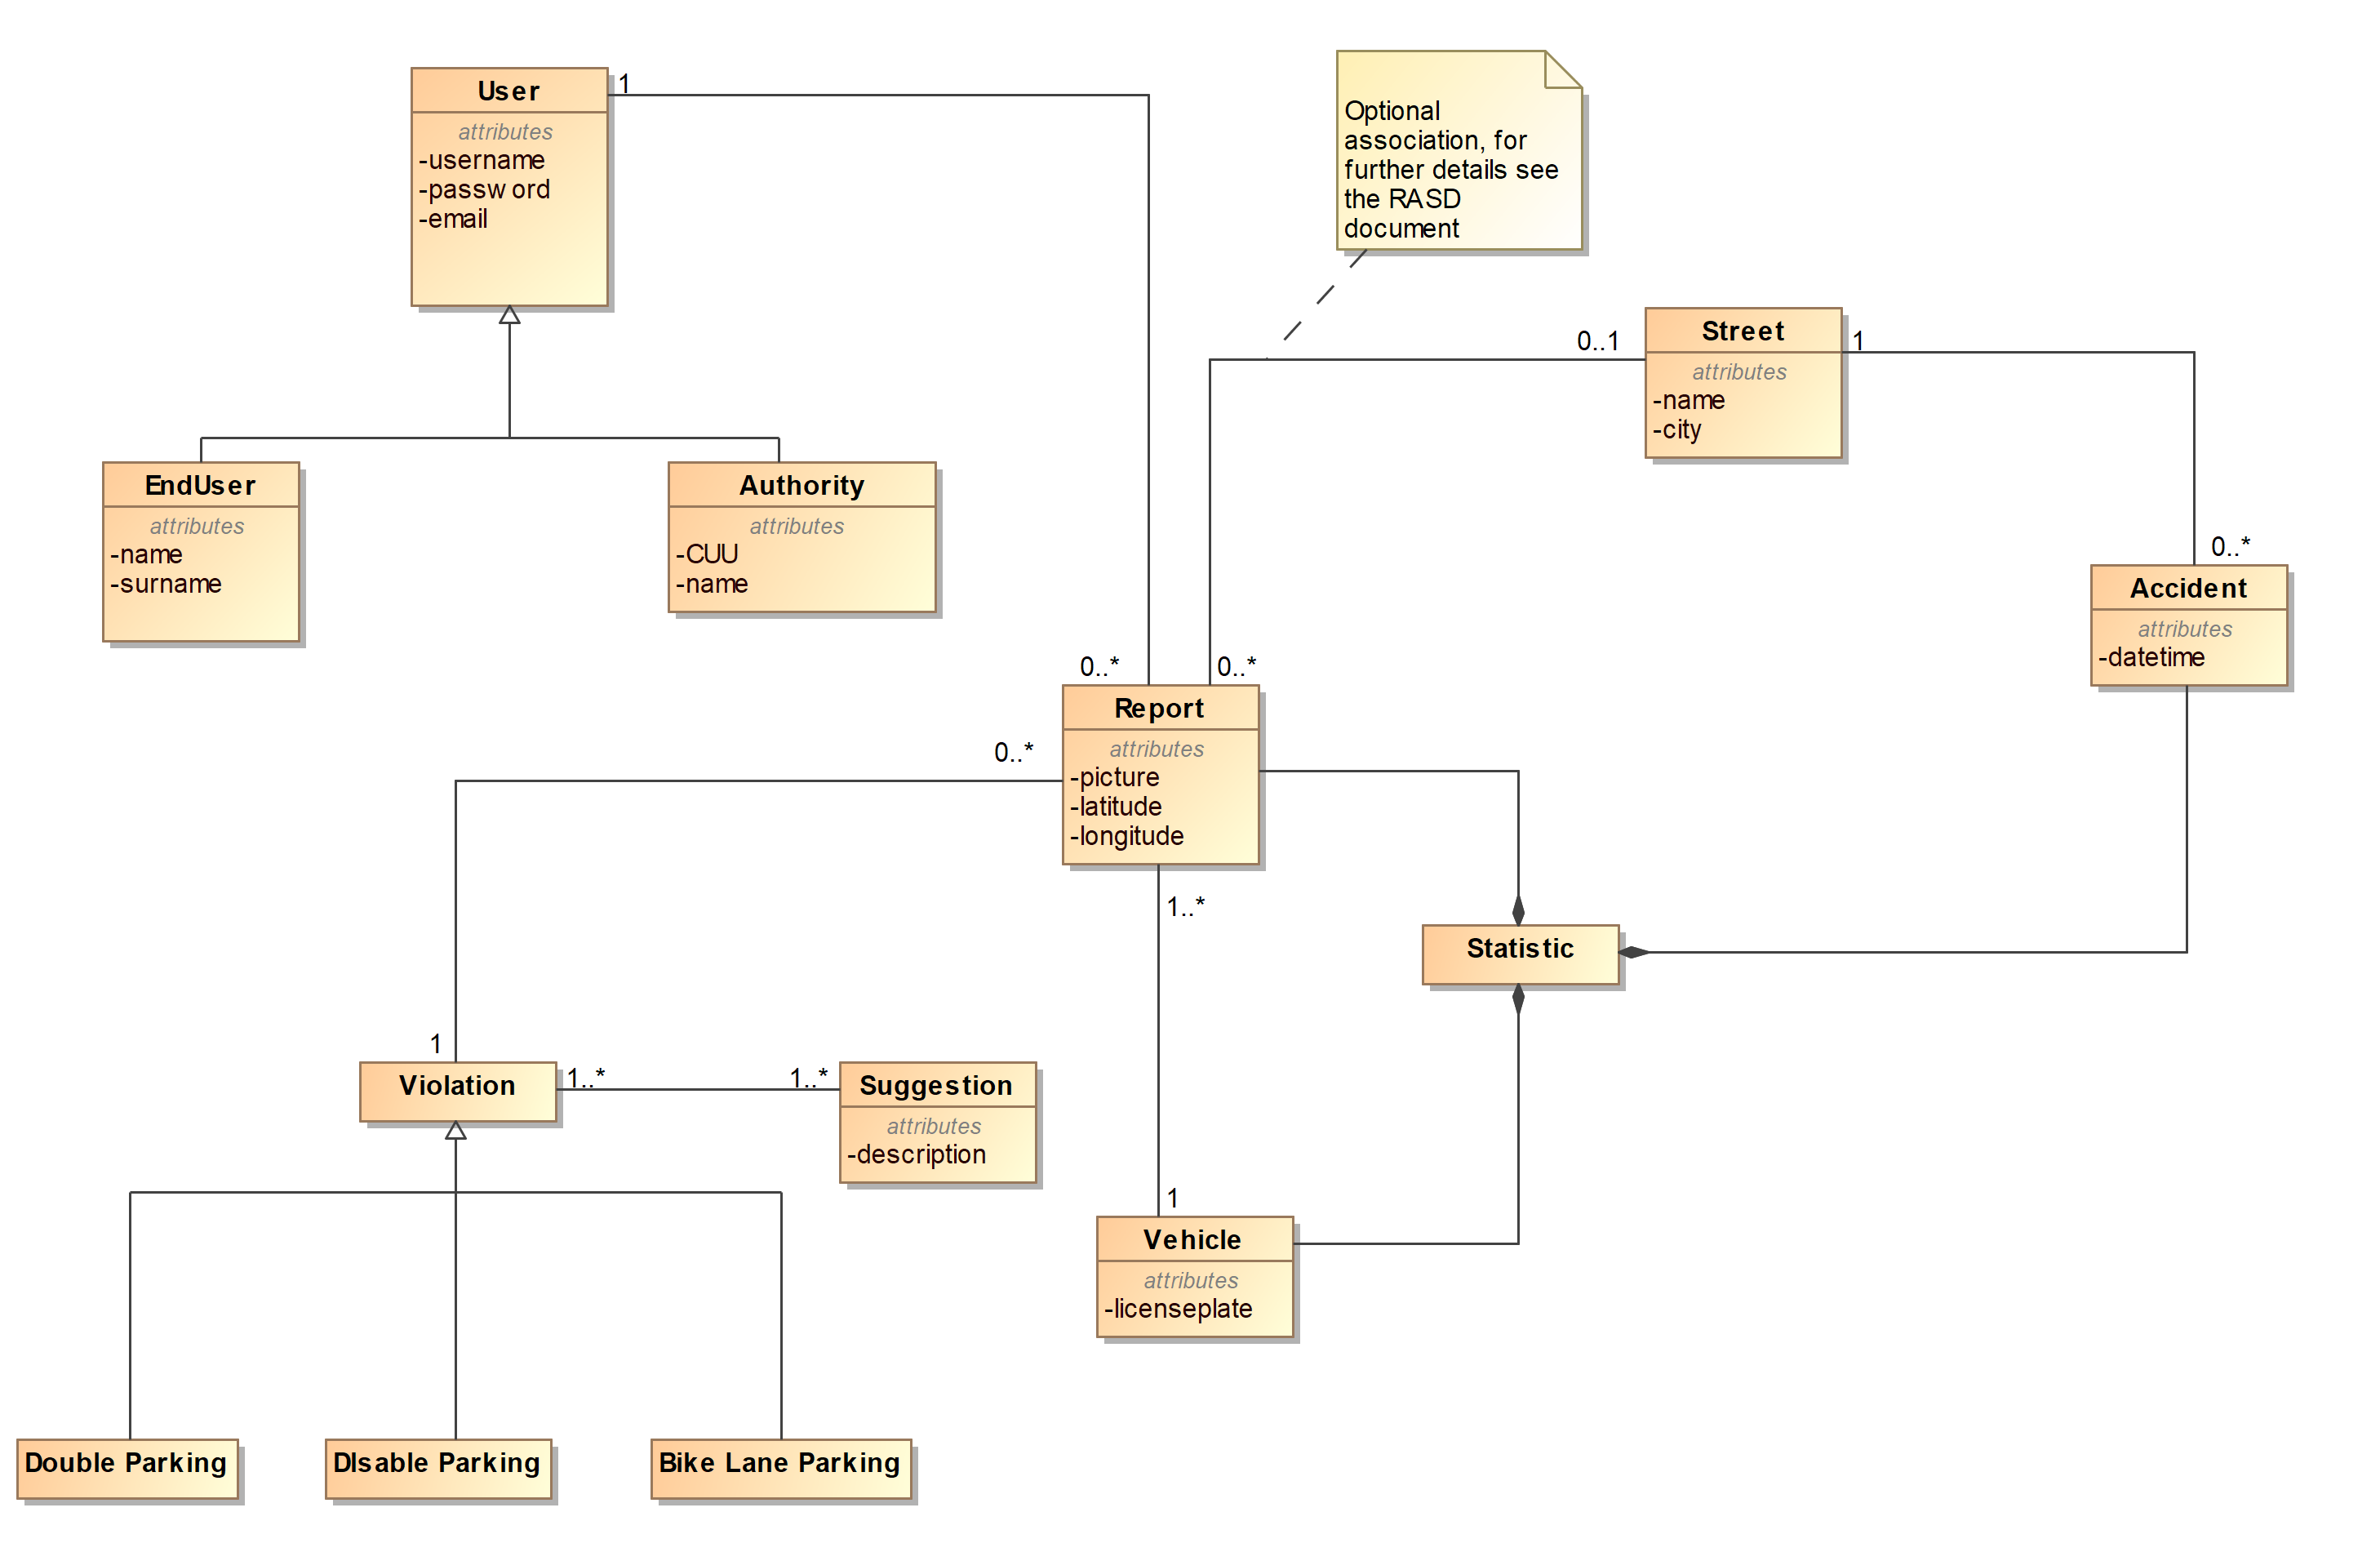
\includegraphics[width=1.12\linewidth]{Images/ClassDiagram.png}
	\caption{Class Diagram}
\end{figure}
The association between Report and Street is optional because we retrieve the position of the report automatically using GPS. Only in case of problem with this operation, we require the address to the user. In this case, SafeStreets calulates the coordinates using the address provided by the user. We use the andress also in case of report made in a place different from the one where the violation occurred. 
\subsubsection{Statechart}
\begin{figure}[H]
	\centering
	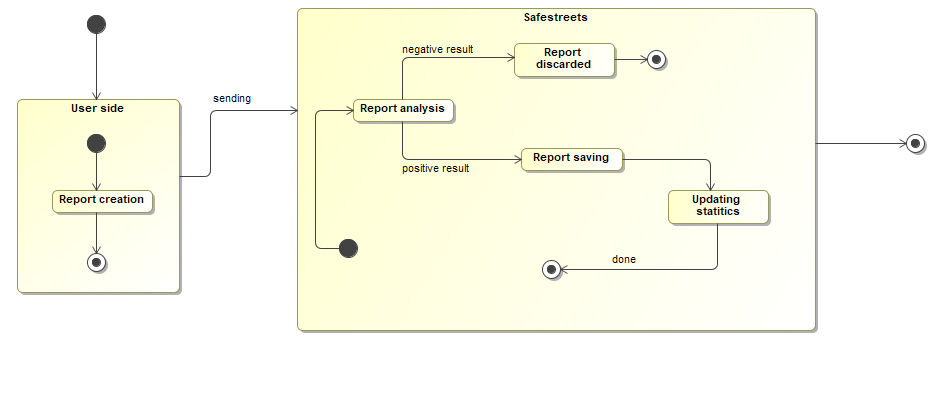
\includegraphics[width=1.12\linewidth]{Images/ReportLifeCycle.png}
	\caption{Report life cycle}
\end{figure}
\begin{figure}[H]
	\centering
	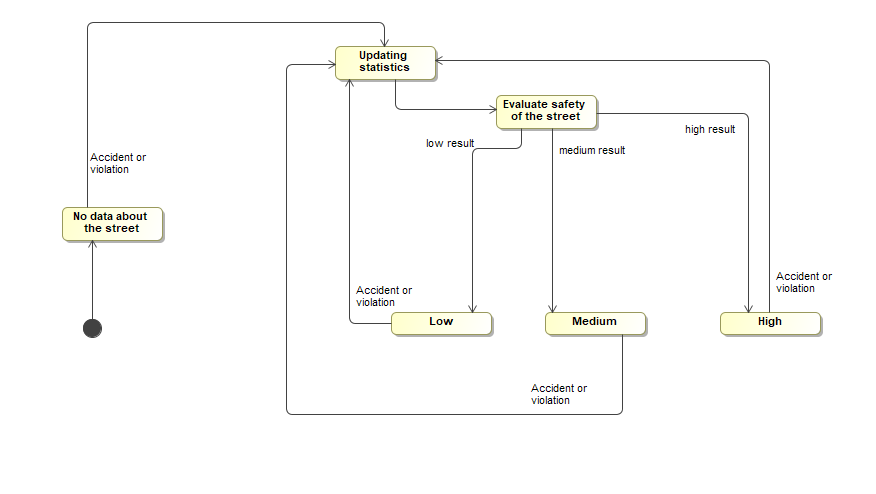
\includegraphics[width=1.12\linewidth]{Images/StreetLifeCycle.png}
	\caption{Street life cycle}
\end{figure}
\newpage

\subsection{Product functions}
Considering the objectives requested by SafeStreets, main functions are described below:

\subsubsection{Notify Traffic Violations RE.1}
The main requirement of the application is to provide users a smart and effortless tool to notify authorities when traffic violations occur.

Users are able to select the type of violation, providing the name of the street, or using their GPS position, and uploading a picture containing the license plate that will be read by an algorithm.

Furthermore, in order to increase the reliability of the system we require the manual insertion of the license plate. When the license will be retried from the image, the result will be compared with the number sended by the user. If the comparison will not return equality, the report will be discarded.

\subsubsection{License Plate Recognition RE.2}
License plate recognition functionality is crucial for SafeStreets, from the license plate we can get information about the owner, the vehicle and its specs.

The fact that there isn't a human being responsible for manually recognizing license plates is important for the scalability, when the application will be used on a large scale.

Automatic number-plate recognition (ANPR) technology consists in seven primary algorithms that the software requires: Plate localization, Plate orientation and sizing, Normalization, Character segmentation, Optical character recognition, Geometrical analysis, Averaging of the recognized values to produce a more reliable or confident result.

Due to the fact that the image will be widely analyzed, it must be in high resolution with no blur and in a good lighting context.

\subsubsection{Data Collection RE.3}
Due to the fact that data is the most valuable asset of modern industry, data collection is important for all statistics, information and data visualization that SafeStreets provides.

It collects data coming from different sources: users inputs, municipality and police databases.
Data collection involve several practices about correctness and security.

\subsubsection{Data Visualization RE.4}
A portion of the application is dedicated to data visualization by showing a map on which the streets/areas are colored according to the frequency of violations and accidents, compared to the average numbers: 
\begin{itemize}
\item red = high
\item yellow = medium
\item green = low
\item white = no data
\end{itemize}

Also there is a part of the UI where authorities can see statistics about vehicles and their violations.

\subsubsection{Data Sets Analysis RE.5}
The functionality of data analysis is crucial for finding patterns in data sets.

\subsubsection{Suggest Possible Interventions RE.6}
Thanks to data sets analysis, SafeStreets can suggest possible interventions for already identified "high-violation" streets.

For each type of violation is assigned one or more possible interventions that will help to decrease the occurrence of that specific violation.


\subsubsection{Information Integrity RE.7}
Data integrity is defined as maintenance and assurance of data consistency over its entire life-cycle.

Ensuring that data are correct and information are never altered is crucial, because local police could take the information about violations coming from SafeStreets.

\subsubsection{Generating Traffic Tickets RE.8}
This functionality is not an internal feature of the application. 

Our scope is to provide the police, data about violations and with this information the municipality could generate traffic tickets with their own systems..

For this reason SafeStreets exposes REST API endpoints to allow authenticated authority users, in this case the police, to get violations information.


\subsection{User characteristics}

The following actors are the users of this application:

\begin{itemize}
	\item End users
\end{itemize}

The end user is a person who, after the sign up, can use SafeStreets to notify traffic violations, consult statistics and see the map with violation information for each street.

\begin{itemize}
	\item Authorities:
	\subitem Municipality
	\subitem Local police
\end{itemize}


Authority is an organization who, after a different sign up from end users, using CUU code, can use SafeStreets to get information about traffic violations for generating traffic tickets, consult possible interventions suggested, see statistics and the map with violation information for each street.
Also they can provide their data to SafeStreets, in this way our platform is able to cross authorities data with its own data.

\subsubsection{Assumptions, dependencies and constraints}
	In this document it is supposed that:
\begin{itemize}
	\item 
	in the country where SafeStreets will be used, the law admits these type of systems.
	
	\item 
	we consider only the following type of violations
	\subitem
	Double parking
	\subitem
	Disable parking
	\subitem
	Bike lane parking
\end{itemize}





\clearpage
{\color{Blue}{\section{Design architecture}}}
\label{sect:overview}
\subsection{Overview}
The architecture we have decided to adopt, is the three-tier architecture.
It is divided into three levels: Presentation, Application and Data Access.

The presentation tier contains the user interface of the web platform, it displays to the end-user the useful data like statistics.

The application level contains the core of the platform, it is composed by: the application server with the application installed and the web server.
It contains the functions that elaborate the data (e.g. Check report validity, LicensePlate export from image).
The application server also allows multiple clients to work simultaneously.

Data access layer contains the database, which store all the reports, streets and users data (end-users and authorities).
Some communications between presentation and application layers are asynchronous.
This structure grants speed because the team can improve every single layer without having impact on the other tiers.
It improves the efficiency because it brings separation between independent tasks.

\begin{figure}
	
	\includegraphics[width=0.95\linewidth, height=0.20\textheight]{../DD/Images/architecture}
	\caption{High­‐level
		system
		architecture}
	\label{High­‐level
		system
		architecture}
\end{figure}
\newpage
\begin{figure}[H]
	\centering
	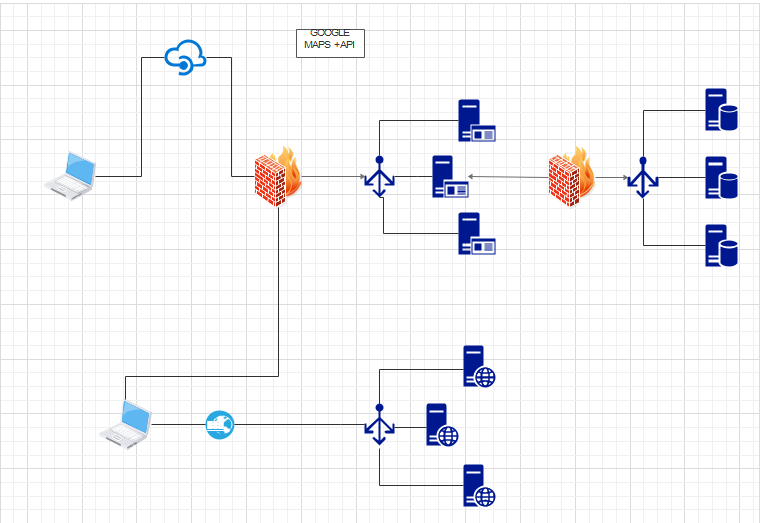
\includegraphics[width=0.98\linewidth, height=0.55\textheight]{Images/networkarchitecture}
	\caption{Network Architecture}
	\label{fig:networkarchitecture}
\end{figure}

The network architecture illustrates how the three-tier is applied to SafeStreets. The presentation level is all information that are shown on the web-app UI.

The authority own systems, that are not incorporated in the SafeStreets system, represent the software used to generate traffic tickets. They receive the data (type of violation, license plate, name, surname etc.) from the API that SafeStreets provides.

The application tier contains the web server and the application server. The web server provides the HTML pages and the JavaScript logic, to the web clients. 

The web server does not communicate with the application server because the contents of the web pages will be filled dynamically with the JavaScript calls between the authority/user device and the application server. 

With JavaScript asynchronous calls the client make and API call to some specific endpoints, by making a \textit{promise}.

The promise is resolved when the client receives data, in our case in JSON format, or the server communicate the HTTP status of the request made.
Contents of the pages can be updated when the JSON object is received.

The data access level contains the database server, that communicates with the application server.
The latter will interrogate the database server to retrieve, update or remove data.

The application server is connected with two firewalls.
They guarantee and improve security of the network and provide more controls on the packets that are sent through the network.

In order to grant better performances, every server is connected to a load balancer to distribute the request avoiding slowdowns.

The end devices exploit the browser cache to grant less requests.

\subsubsection{Database structure}
The database will have a structure according to the following one: 

\begin{figure}[H]
	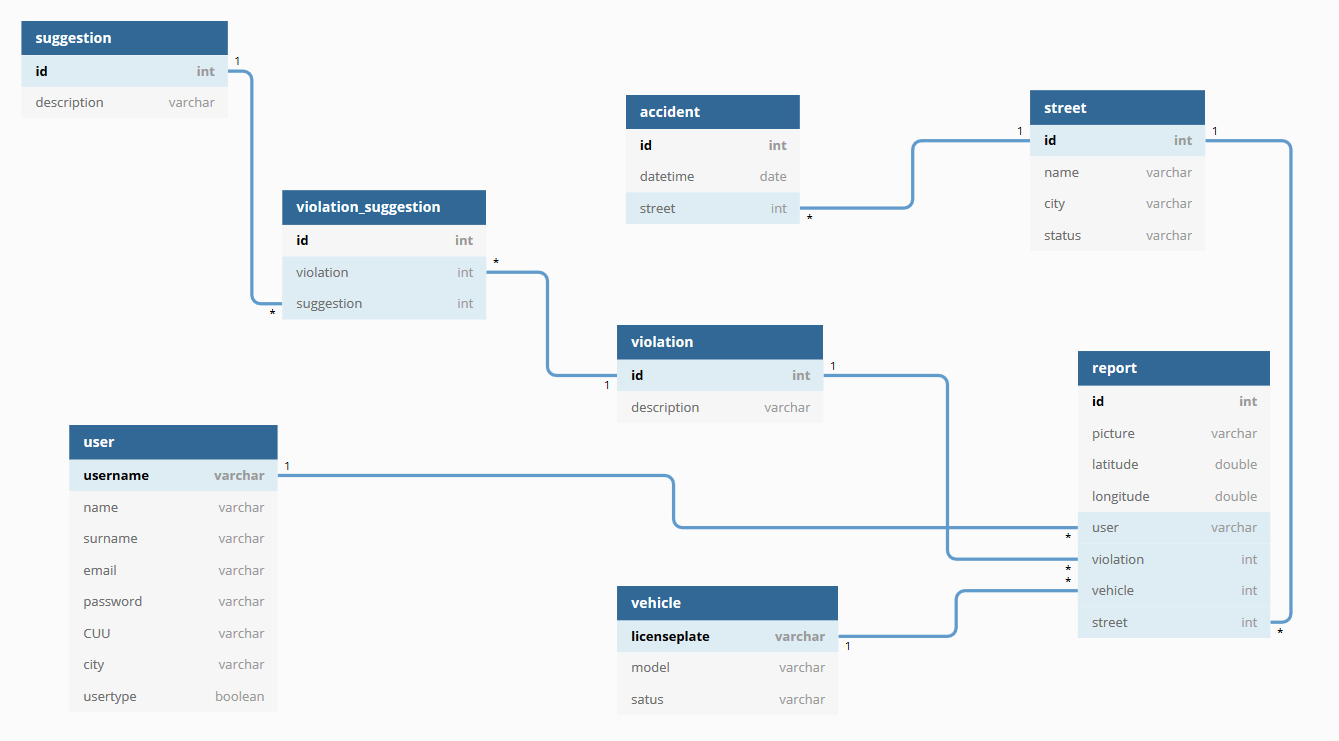
\includegraphics[width=0.95\linewidth, height=0.50\textheight]{../DD/Images/ER}
	\caption{Database structure}
	\label{Database structure}
\end{figure}


\subsection{Component view}
In order to give a better description of the component of the system, the class diagram below shows how the application is designed.

All this description regards only the application tier of the system.

Communication between client and the application is made by an interface exposed (SystemMangerInterface).
 
The client, used by end users and authorities that want to see statistics, does not contain any portion of the logic of the system (except for the GPS tracking). 

Thus it is a thin client and no class diagram has been made for it.

In diagram notes, it is possible to see which design patterns has been implemented (facade and singleton).

The data are stored in the database, are accessible using the manager classes. Their function is to query the database and save the data retrieved in the appropriate objects (for every entity of the database a specific class has been designed).

All the request arriving from clients are managed by the application server. Then it calls the appropriate method of facade class SystemMananger using the interface SystemMangerInterface. This class uses the methods of other classes to respond to the request.

A SystemManager method, used for obtaining information about accidents occurred, is called periodically. It retrieves the information and then stores them in the database.

During the registration process of an authority the specific method calls a web service to check the authenticity of the CUU code.

Moreover, an interface is exposed to authorities systems. In this way they can call a method that provide the reports data and generate traffic tickets on them. 

Before sending any type of information the identity of the authority is checked using the appropriate method of UserManager class.

\begin{figure}[H]
	\centering
	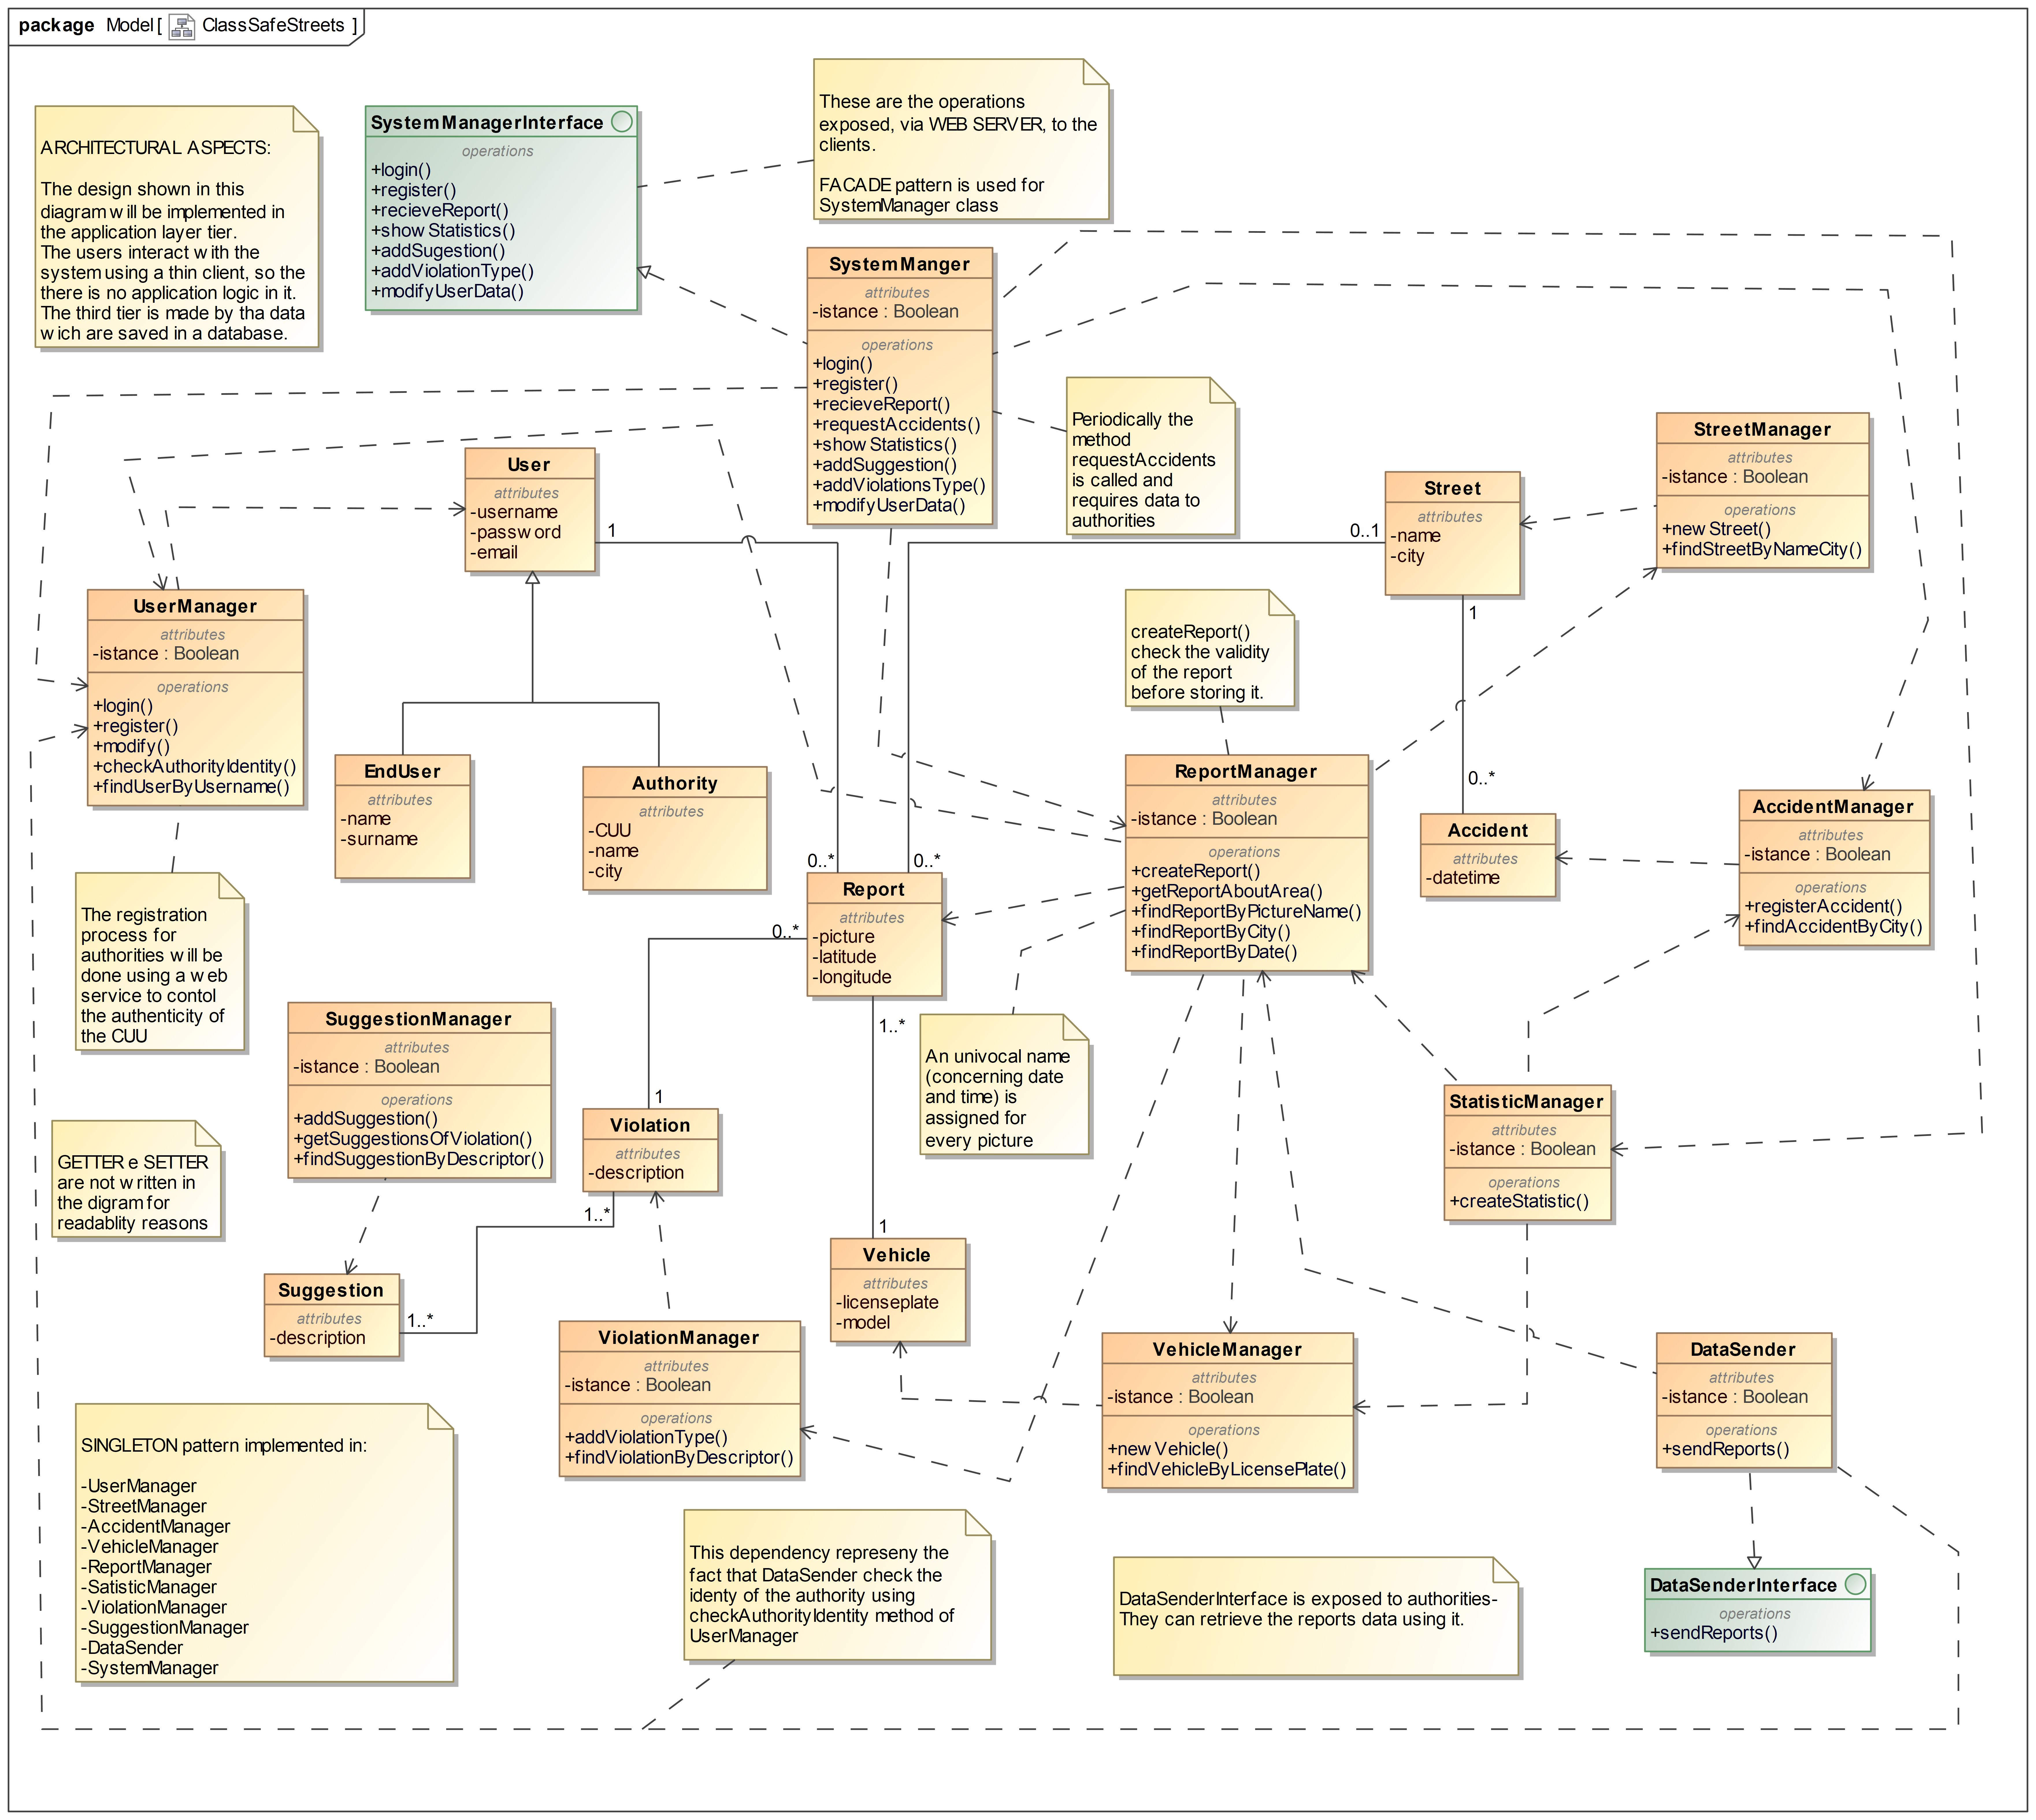
\includegraphics[width=1.12\linewidth]{Images/ClassSafeStreets.png}
	\caption{Class diagram}
\end{figure}

The component diagram below describes the implementation of the classes described before in terms of components.

The macro-component \textit{SafeStretsApplication} represents the Java application running on the application server. It exposes two interfaces: the first one is designed to communicate with the client. The second is exposed to authority systems in order to offer information that can be used to generate traffic tickets.

There are also sub-components that perform specific operations and interact with the database:
\begin{itemize}
 \item 
 SystemManager: is the component that conveys all the requests to appropriate sub-components and periodically activates the AccidentManager.
 \item 
 AccidentManager: is the component that calls the specific service to retrieve the data about accidents occurred. These information will be used by StatisticManager.
 \item
 StatisticManager: is the component designed to create statistic crossing data coming from report and accidents.
 \item 
 PositionManager: is the component used to organize data about position and streets.
 \item 
 UserManager: is the component used to manage user operations (for instance login,registration...).
 \item
 ReportSender: it is used to send data about reports stored to authority system. These information will be used to generate traffic tickets. This sub-component exposes directly an interface to the external environment. Naturally before sending the data, the method check the identity of the authority using the UserManager.
 \item 
 VehicleManager: is the component designed to manage the data about vehicle.
 \item 
 ViolationAndSuggestionManager: it is used to store and modify the type of violation and suggestion.
 \item 
 ReportManager: is the component that store reports in the database and retrieve information on it.
 \item 
 DatabaseManager: it is used to keep the connection to the DBMS and to send queries to it.
 
\end{itemize}

\begin{figure}[H]
	\centering
	\includegraphics[width=1.12\linewidth]{Images/component.png}
	\caption{Component diagram}
\end{figure}

\subsection{Deployment view}
In the deployment diagram below it is possible to see the physical implementation of the system.
SafeStreets is composed by 3 nodes:
\begin{itemize}
	\item 
	First tier: represent the thin client that make HTTP requests. It is used by users for sending reports and by authorities in order to see statistics.
	\item 
	Second tier: is made by the web server and the application server. The first one is responsible of the catching of the HTTP requests coming from the clients. The web server read the requests and call the appropriate method exposed by the application server. The real computation of the requests is done here.
	When data stored are required, the application server communicates with the third tier.
	\item 
	Second tier: this tier represents the database of the system. 
\end{itemize} 

In the diagram there is also another node that corresponds with the authority system in charge of retrieving reports to generate traffic tickets. The application server exposes a interface that provides this function. 

\begin{figure}[H]
	\centering
	\includegraphics[width=1.12\linewidth]{Images/Deployment.png}
	\caption{Deployment diagram}
\end{figure}

\subsection{Runtime view}
\newpage

\subsubsection{End-user registration}
The sequence diagram below shows how it is developed the registration of a new user. The SystemManager class , through its interface, calls  the method "register()" of the UserManager, giving three parameters: username, mail, password. The first two parameters must be unique otherwise the registration failed.
UserManager will call the method "insert()" of DatabaseManager that will recieve the query to insert the User into the database.
\begin{figure}[H]
	\centering
	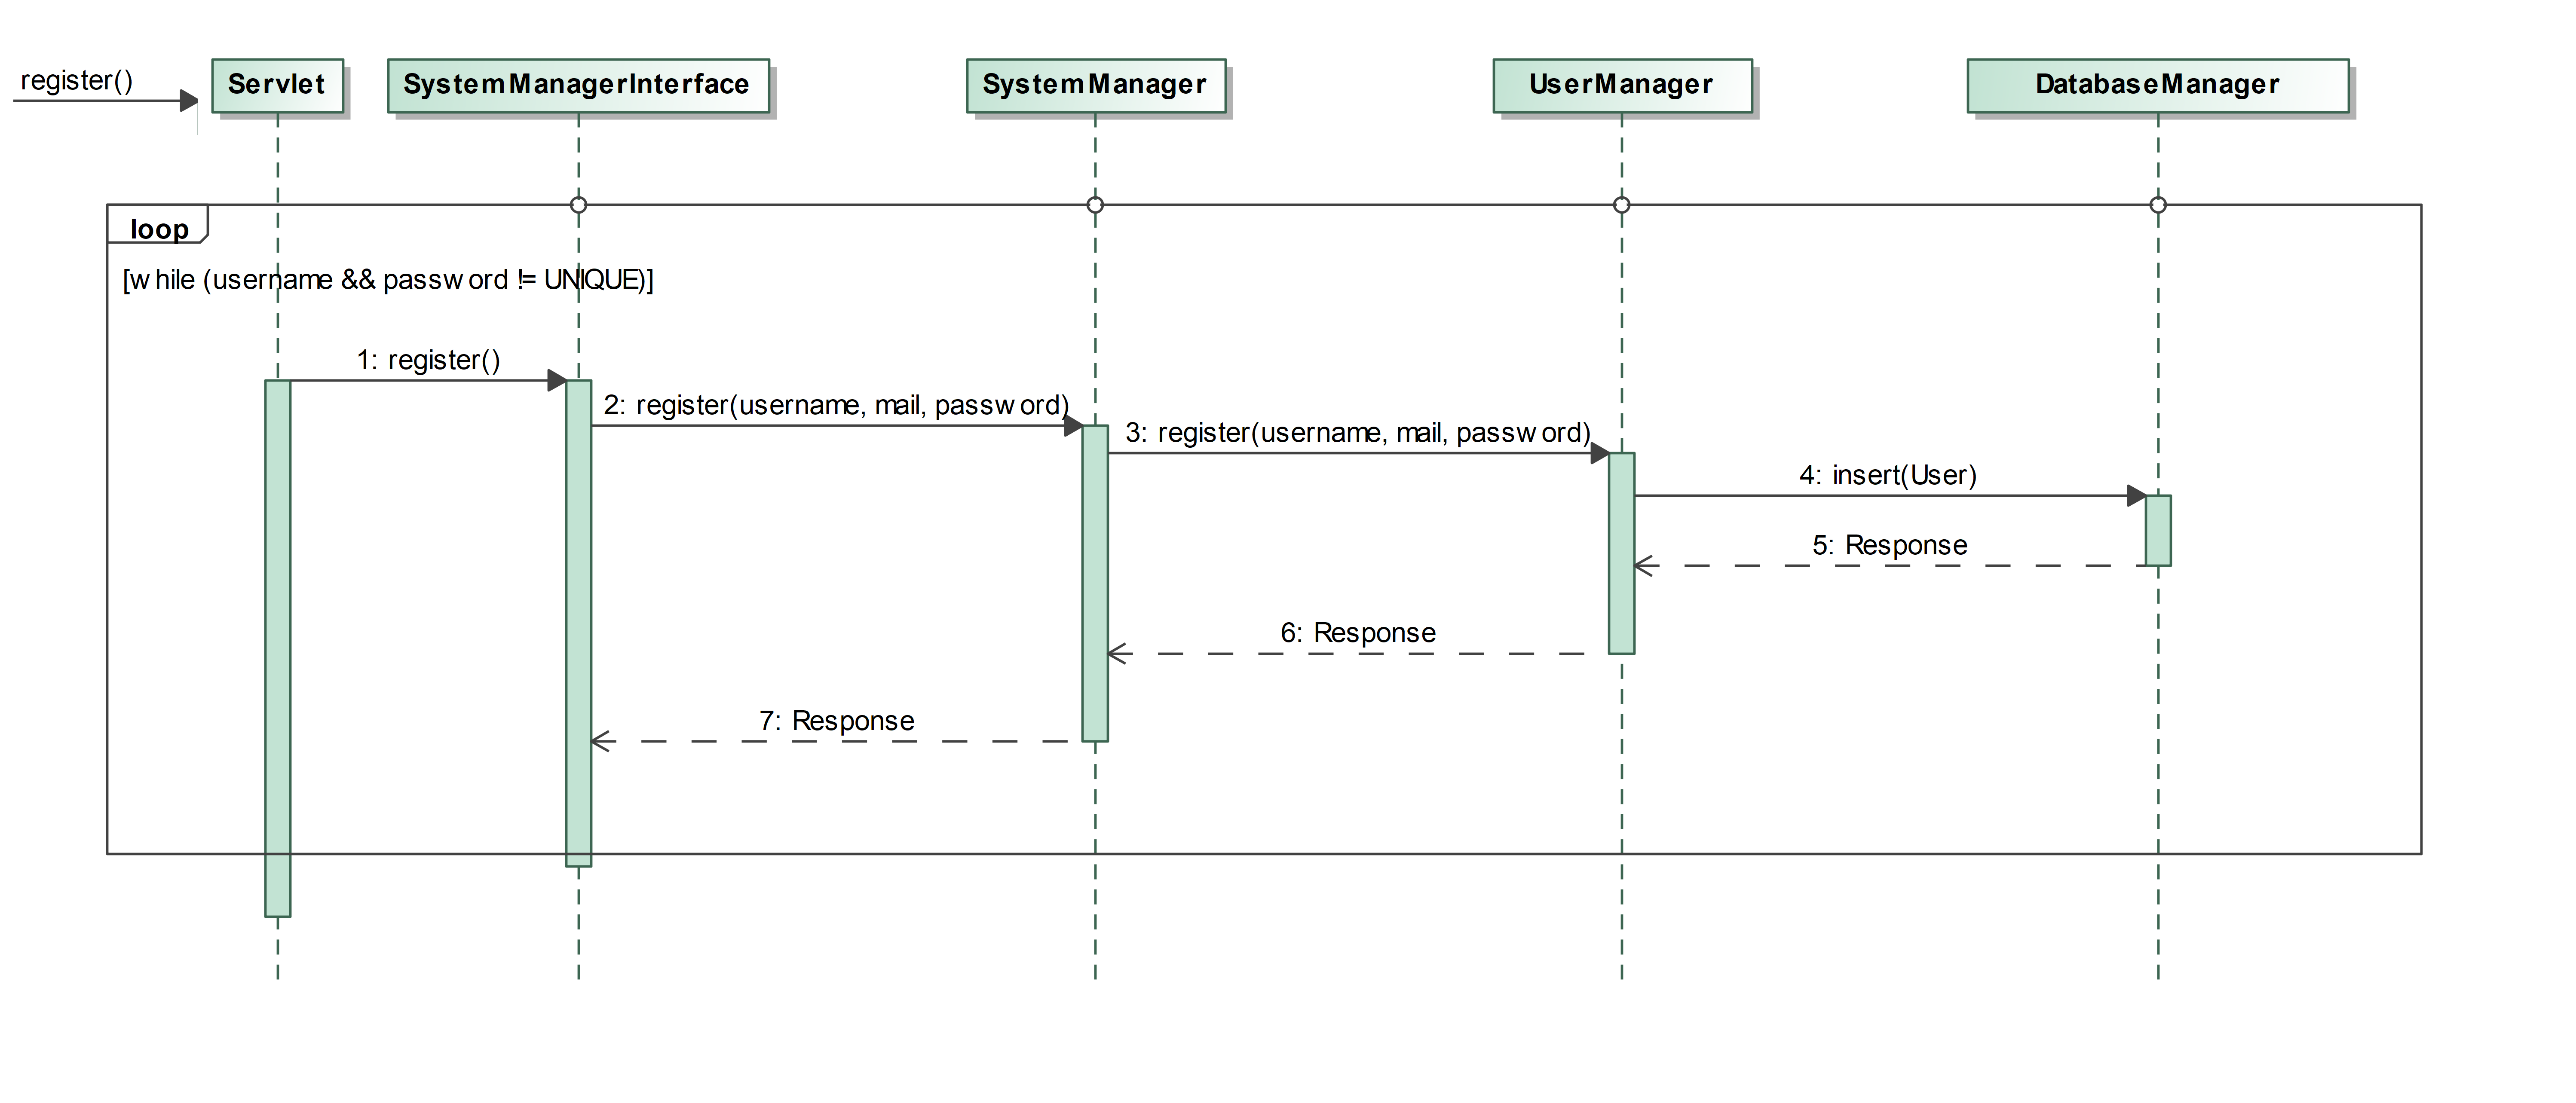
\includegraphics[width=0.97\linewidth, height=0.32\textheight]{Images/RunTimeDiagram/Sequence1}
	\caption{Register}
	\label{fig:Register}
\end{figure}
\subsubsection{User reports a violation}
 SystemManager calls the method createReport() that will create a Report object with the data received. The report is created and stored only if it is valid and consistent. 
 
Once the report is received, if they are not already present in the database, the street and the vehicle will be added in the database, through DatabaseManager, using the different manager, StreetManager and VehicleManager with respectively: newStreet() and newVehicle().
\begin{figure}[H] 
	\centering
	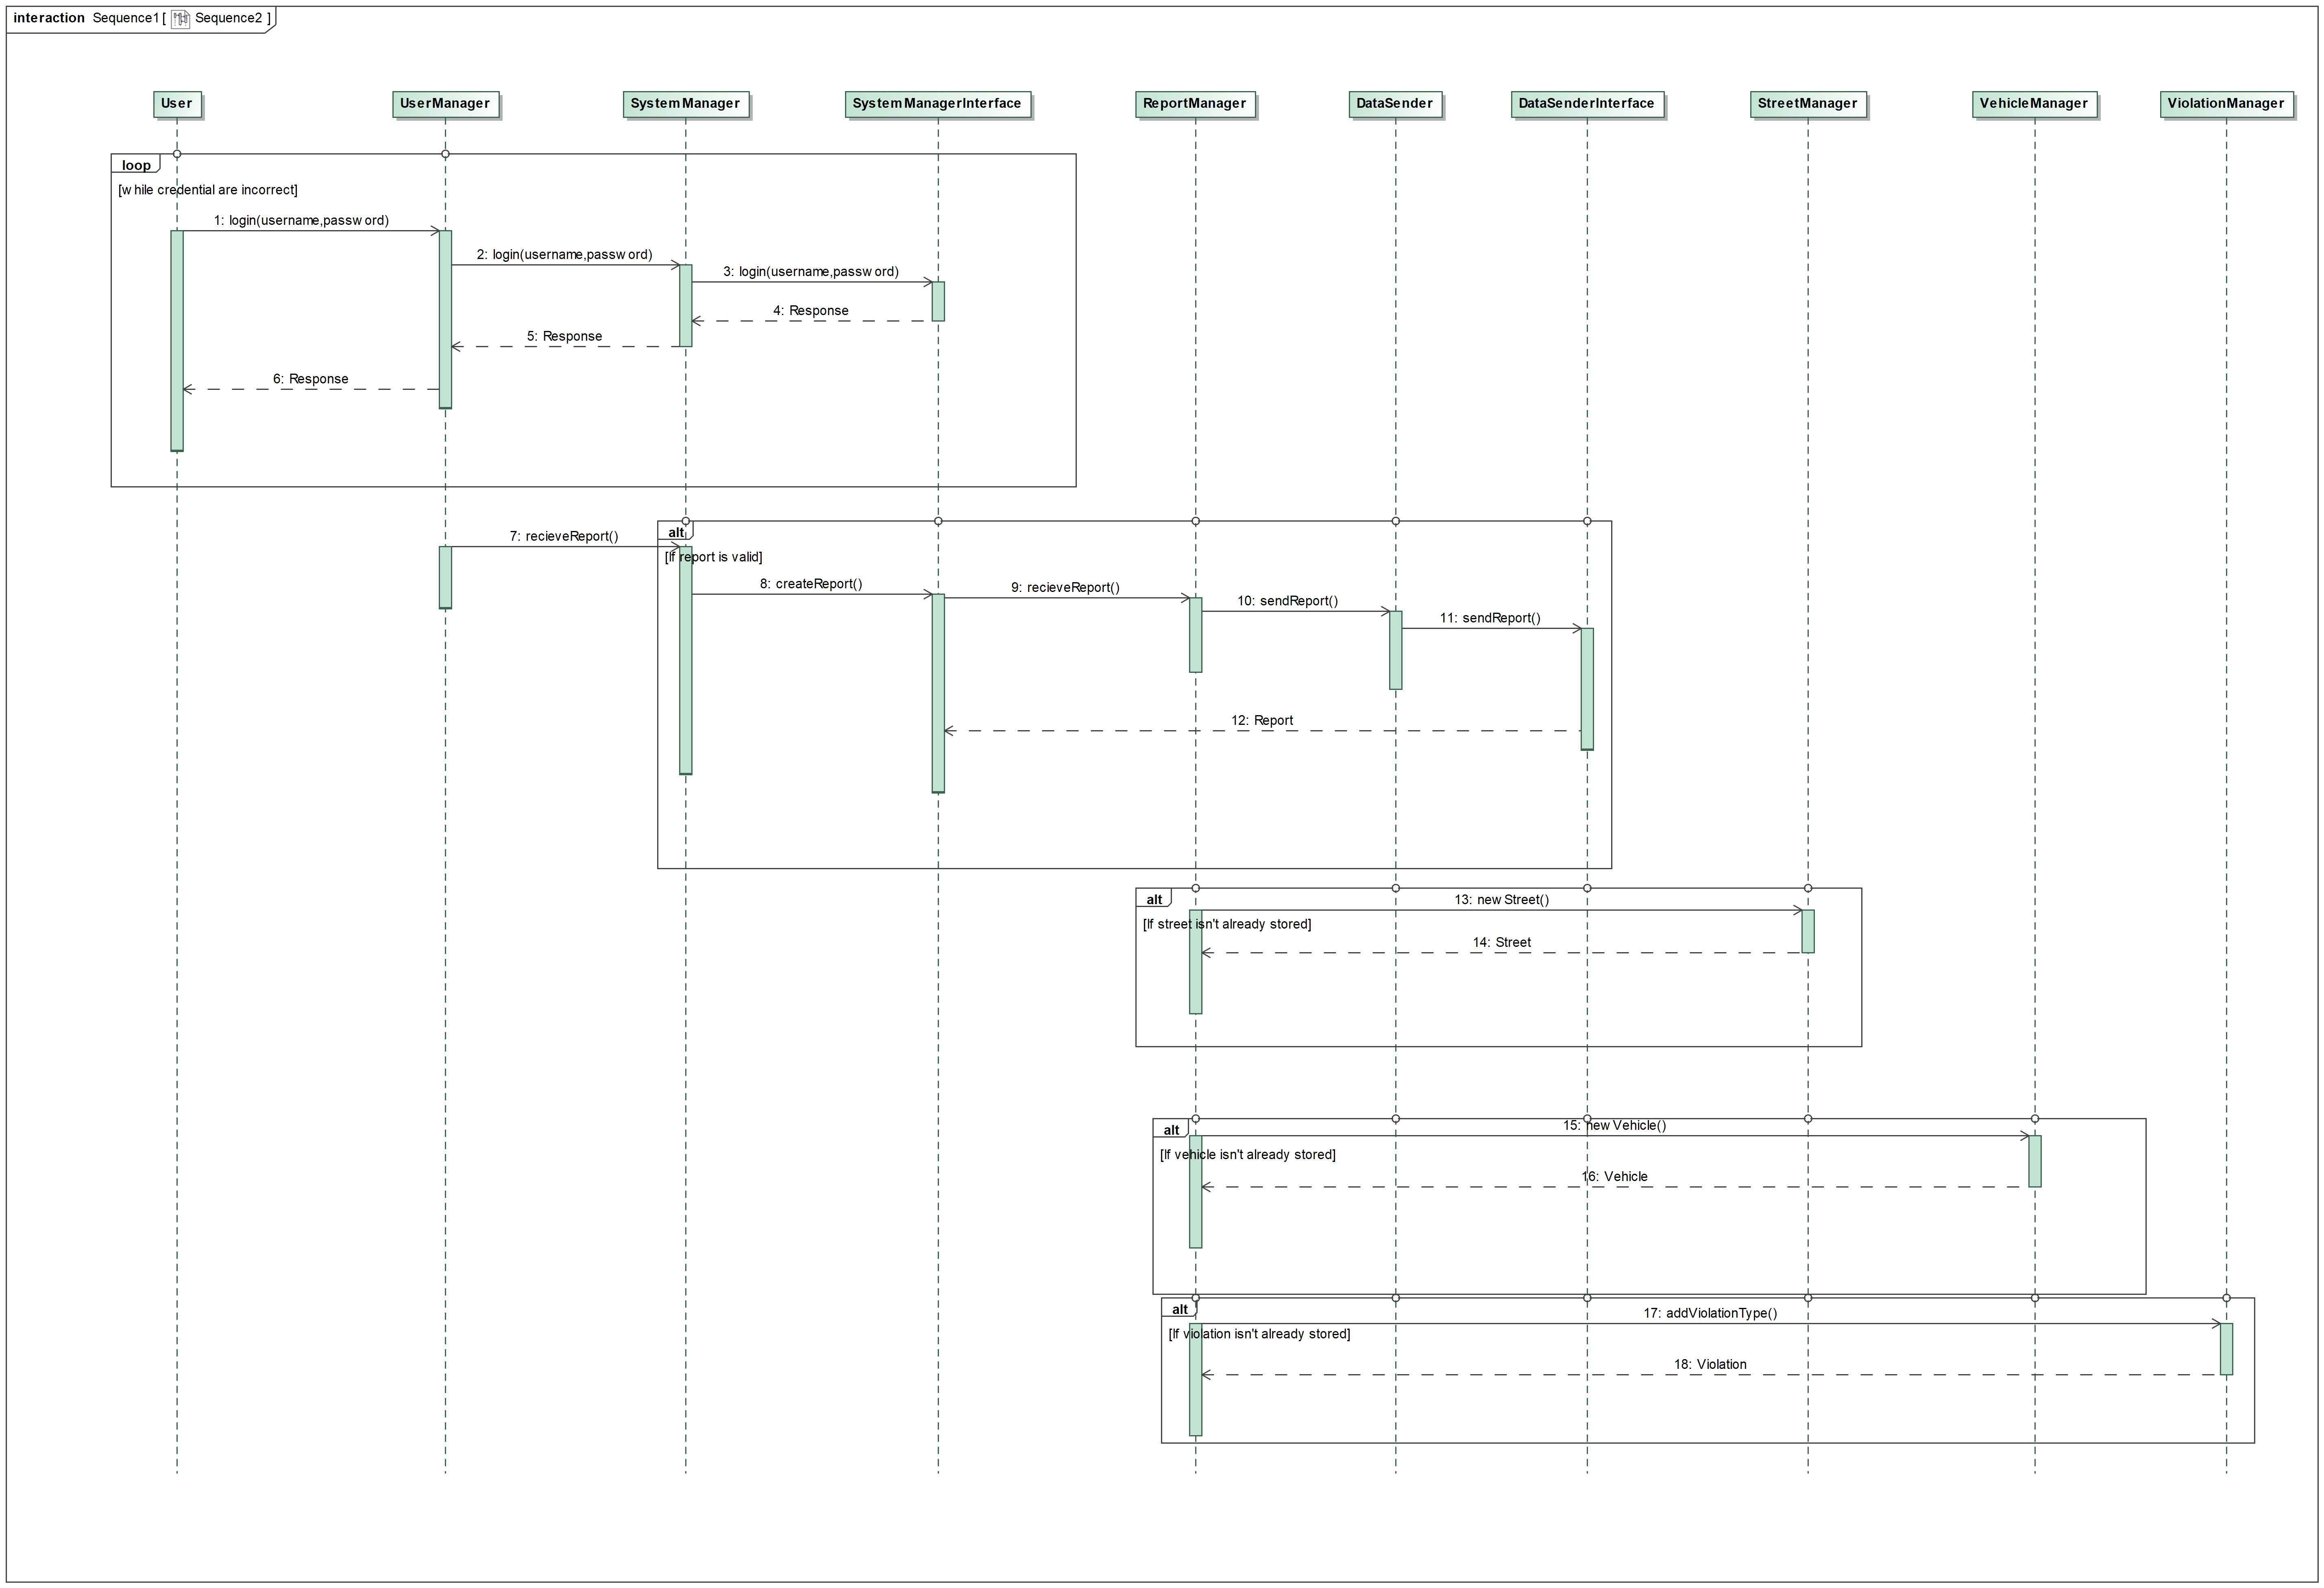
\includegraphics[width=0.95\linewidth, height=0.7\textheight]{Images/RunTimeDiagram/Sequence2}
	\caption{User reports a violation}
	\label{fig:User reports a violation}
\end{figure}

\subsubsection{Generate statistic}
SystemManager receives the client call showStatistic() and will uses the method createStatistic() of StatisticManager class.

This method uses DatabaseManager to retrieve data from the database and generate statistics regarding a specific area.

Statistic contains: information about number of violations and accidents, most unsafe areas and most involved vehicles.
\begin{figure}[H]
	\centering
	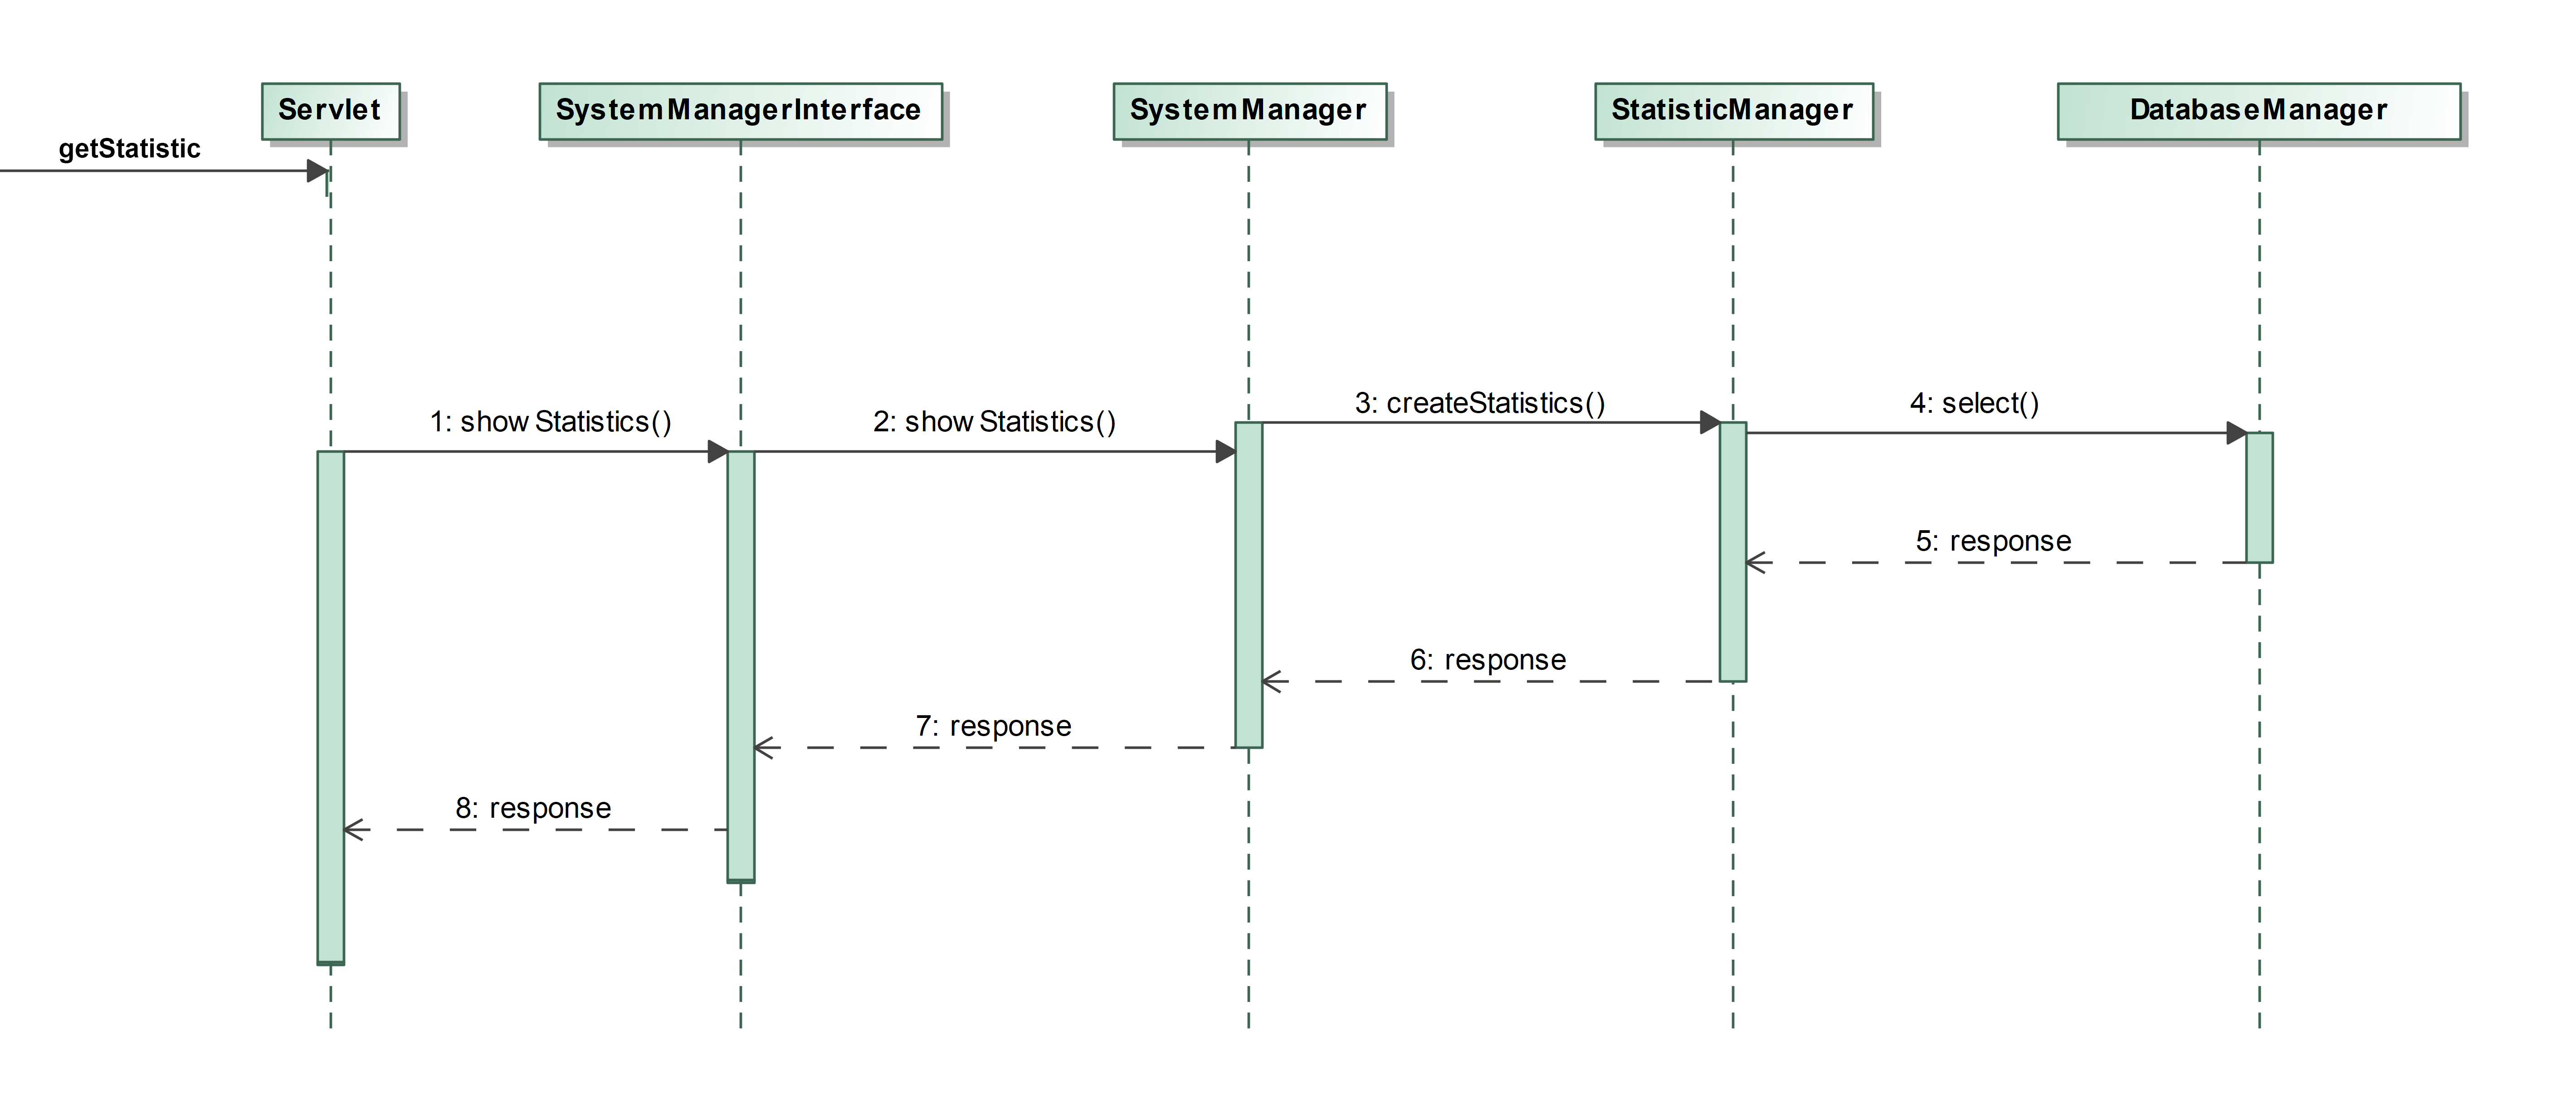
\includegraphics[width=0.97\linewidth, height=0.35\textheight]{Images/RunTimeDiagram/Sequence4}
	\caption{Insert accident and generate statistic}
	\label{fig:Insert accident and generate statistic}
\end{figure}
\subsubsection{Check street status}
SystemManager is called by the method streetStatus and uses a proper method of StreetManager to retrieve the information about the status of the street in a specific area. In this process is involved also DatabaseManager that communicates with StreetManager, which receives the data from the database.
\begin{figure}[H]
	\centering
	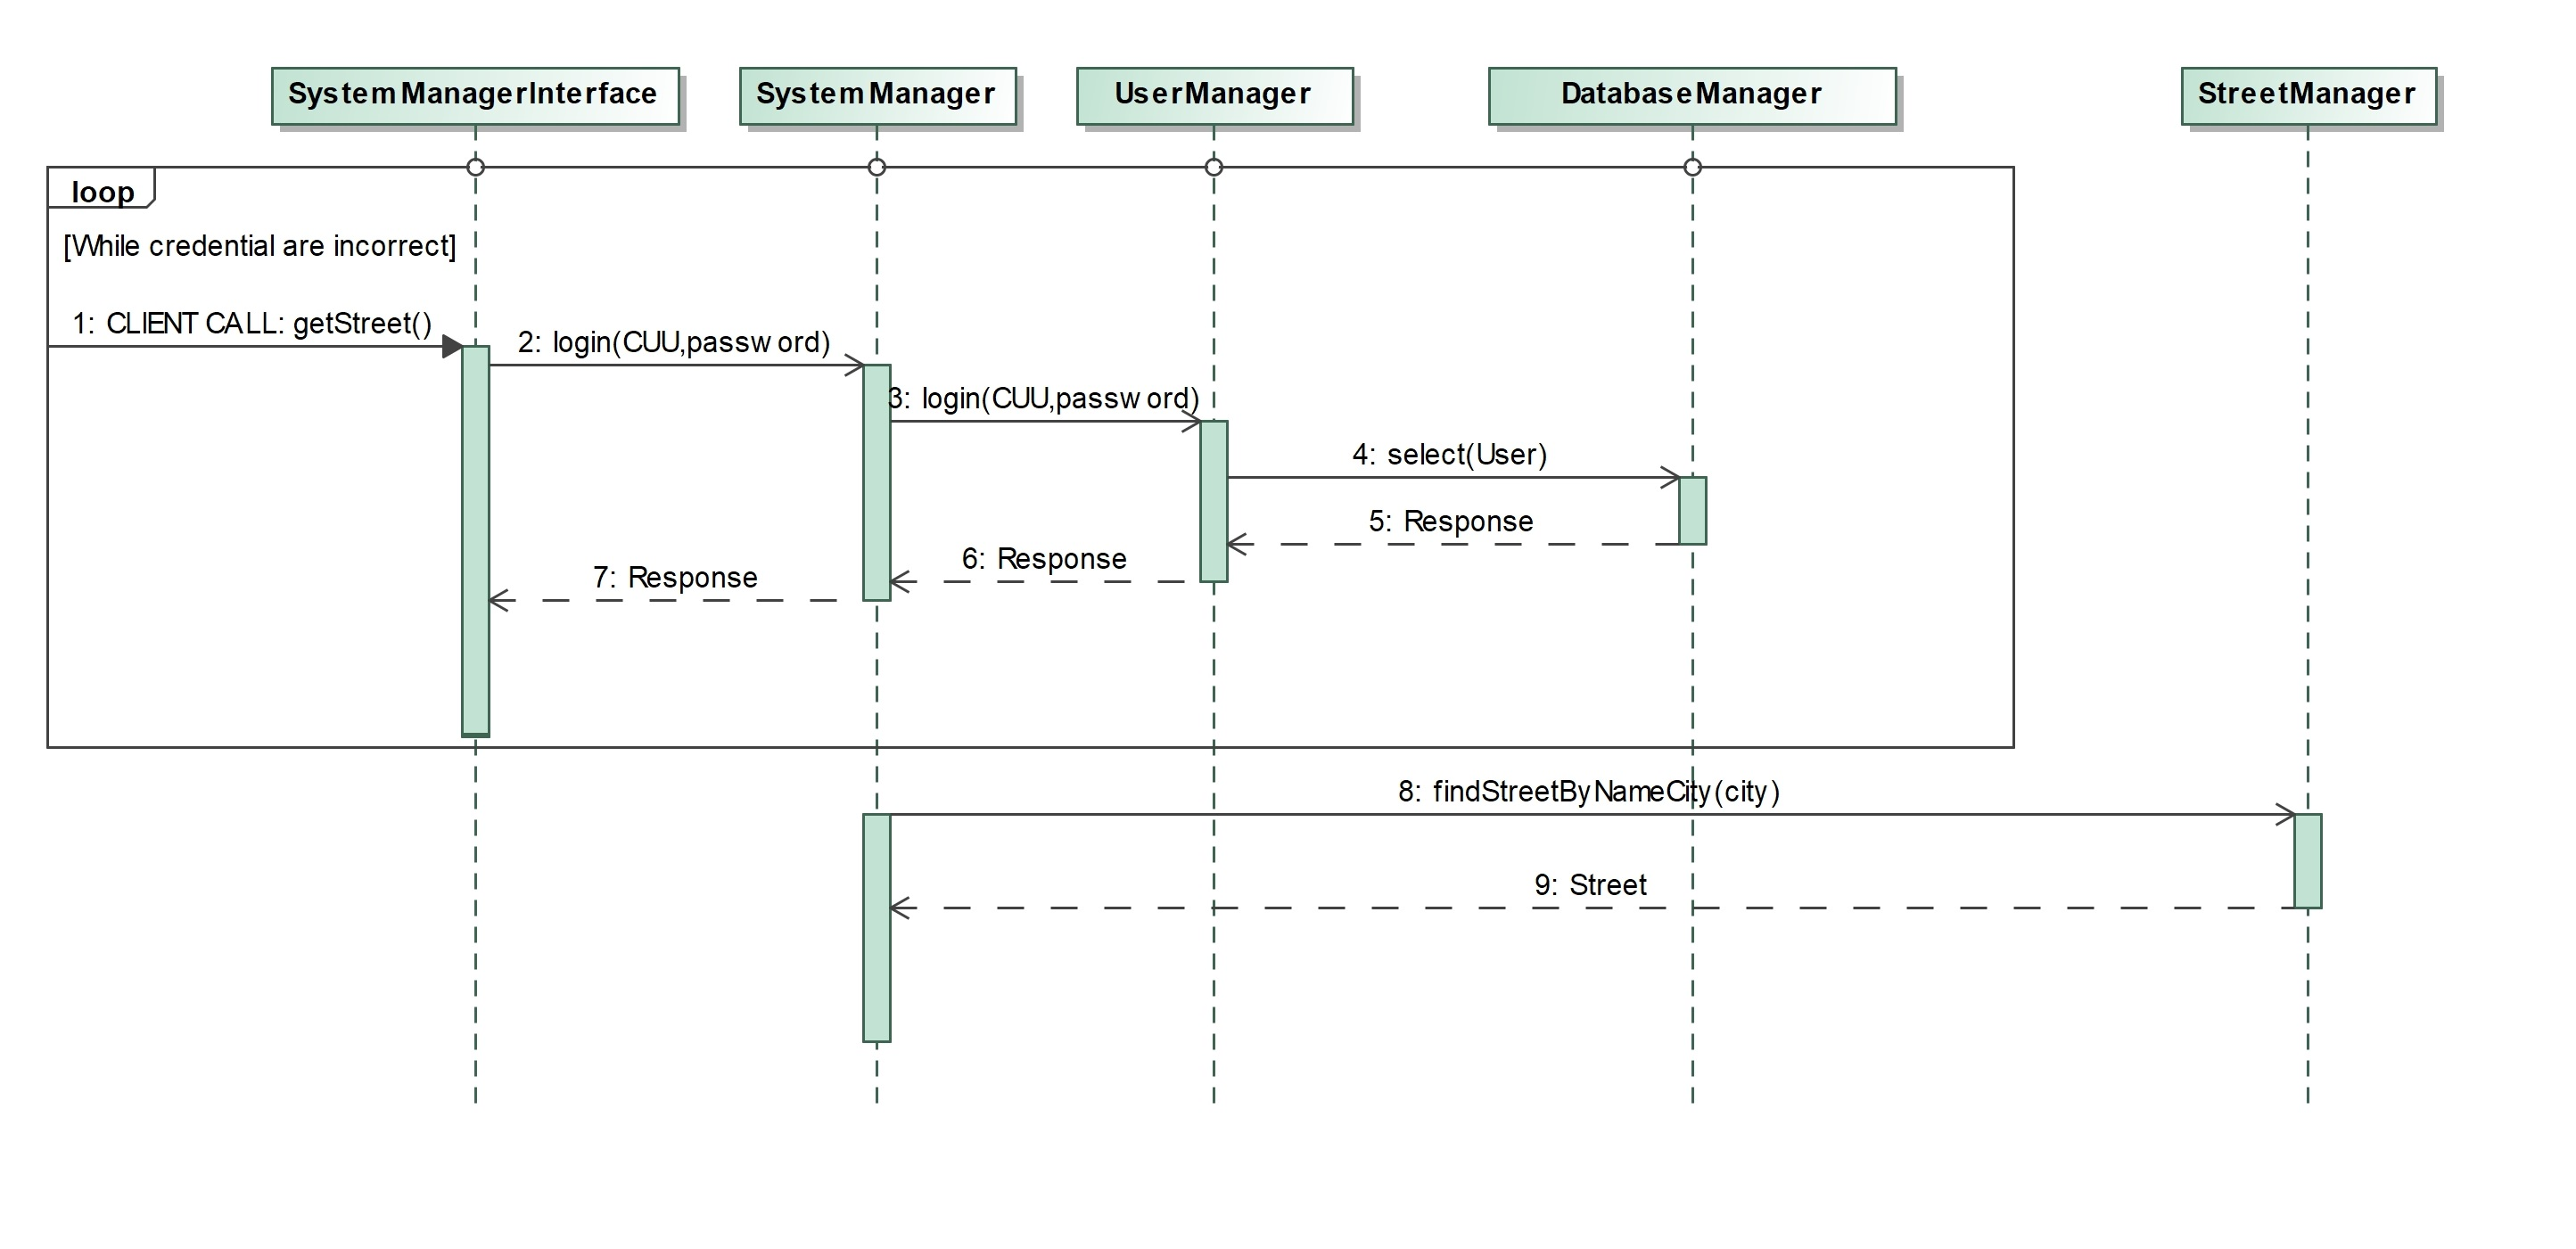
\includegraphics[width=0.95\linewidth, height=0.35\textheight]{Images/RunTimeDiagram/Sequence5}
	\caption{Check street status}
	\label{fig:Check street status}
\end{figure}

\subsubsection{Data sender to Authority}
DataSender receives an external call from the authority own system, the latter is in charge of the generation of traffic tickets. DataSender calls getReportAboutArea() of ReportManager, which returns the reports received in a specific area. 
\begin{figure}[H]
	\centering
	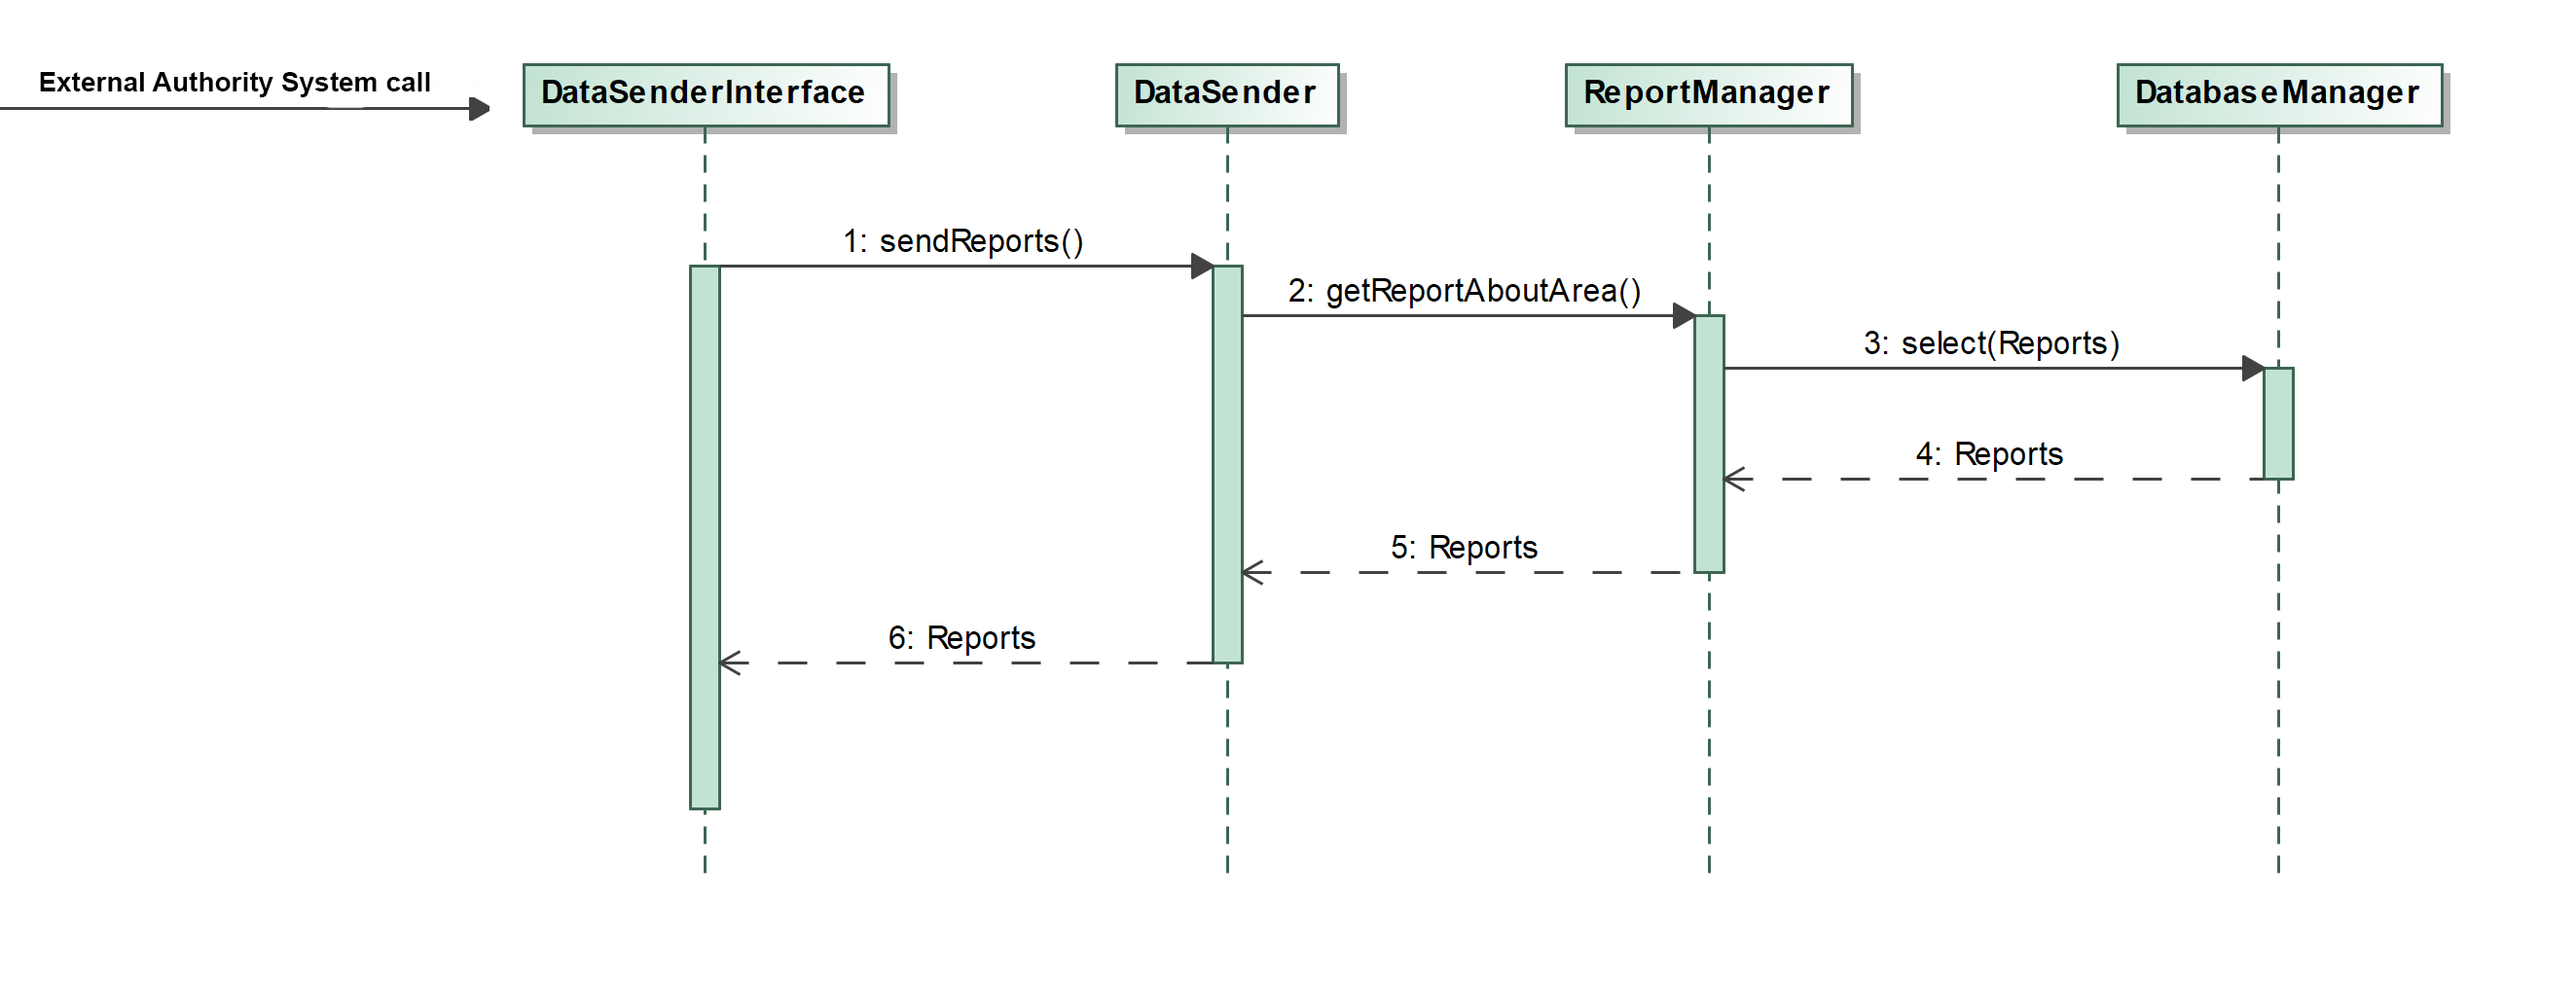
\includegraphics[width=0.9\linewidth]{Images/RunTimeDiagram/DataSender}
	\caption[Data Sender to Authority]{}
	\label{fig:datasender}
\end{figure}


\subsection{Component interfaces}

The interfaces exposed are mainly two: SystemManagerInterface and DataSenderInterface. Their role was explained in the previous sections of this document.

\begin{figure}[H]
	\centering
	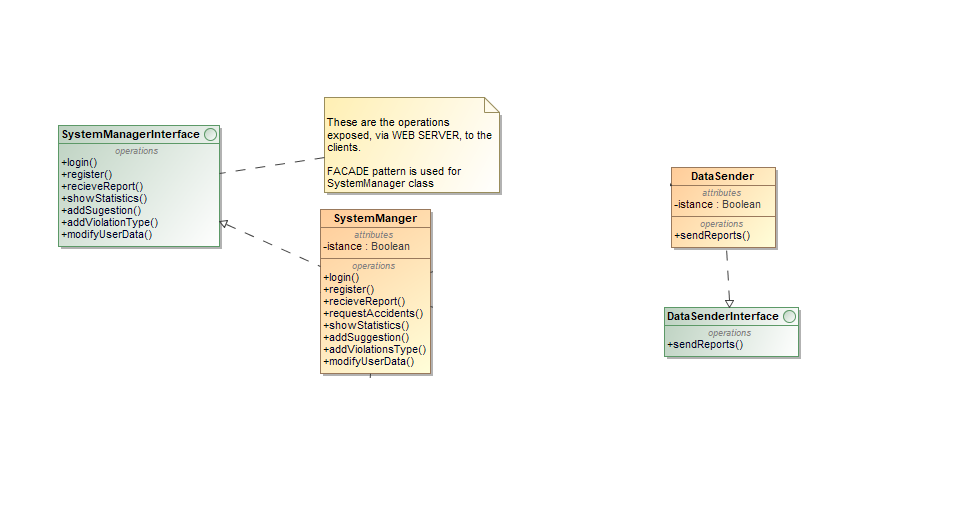
\includegraphics[width=1.12\linewidth]{Images/ComponentInterfaces.png}
	\caption{Component interfaces}
\end{figure}


Here the focus is on the feature provided by the methods exposed.

\subsubsection{SystemManagerInterface}
Every method exposed by this interface will correspond to a servlet that is able to catch the request and return data to the client.
\begin{itemize}
	\item 
	User login(String user, String password)
	
	It is the method in charge of checking the identity of the user/authority that want to log in the application. It returns the object User if the login process was successfully done, otherwise the object is null. 
	
	The application server checks the type of User object returned and then generates the proper response.
	The method works by invoking methods of UserManger class.
	
	\item 
	User register(String user, String password, String mail, String name, String surname)
	
	This method does the registration of a normal user and returns the User object as login method. Since the username has to be univocal the process can abort, in this case a null object is returned.
	Reading the returned object, the application server will generate the proper response.
	The method works by invoking methods of UserManger class.
	
	\item 
	User register(String user, String password, String mail, String name, String CUU, String city)
	
	This method does the registration of an authority user and returns the User object as login method. Since the username has to be univocal and the CUU is checked here (via Web Service), the process can abort, in this case a null object is returned.
	Reading the returned object, the application server will generate the proper response.
	The method works by invoking methods of UserManger class.
	
	\item
	 Bool recieveReport(String picture, Double latitute, Double longitude, String Violation, String violation, String licenseplate, String user, String city, String streetName)
	 
	 This method creates the report. During this process all the checks concerning the authenticity of the picture are performed and the coordinates are transformed into street name and city. In case the operations ends successfully, the proper objects (Report, Vehicle, Street) are created or associated (Violation, User) and then all data will be stored in the database. The picture name will be renamed with an univocal key made on date, time and user. A true value is returned.
	 In case of bad result on the checks of the authenticity, a false value will be returned.
	 According to the value returned by the method, the application server will generate the proper response. 
	 These operations will be performed using methods of ViolationManager, UserManager, ReportManager, VehicleManager and StreetManager.
	 
	 \item
	List<Integer> showStatistics (String user, String city)
	
	This method before generating statistics regarding the city, checks the identity of the user. 
	If the username does not correspond to an authority, it returns a null value.
	Otherwise it generates statistics using data of reports and accidents referred to the city.
	According to the result of the method the application server generates the proper response.
	This method works using UserManager and StatisticManager classes.
	
	\item 
	Bool addSuggestion (String user, String description)
	
	This method before adding the suggestion, checks the identity of the user. 
	If the username does not corresponds to an authority, it returns a false value.
	Otherwise it adds the suggestion into the list and returns true.
	According to result of the method the application server generate the proper response.
	This method works using UserManager and SuggestionManager classes.
	
	\item 
	Bool addViolationType(String user, String description)
	
	This method has the same behavior of the previous one regarding the suggestions.
	
	\item 
	Bool modifyUserData(String oldPassword, String email, String newPassword)
	
	The method updates the data if the username exists and the old password is correct, then
	a boolean value is returned. According to result of the method, the application server generate the proper response.
	The method use UserManager class to perfom that opertaion.
	
	\item
	List<String> streetStatus(Street city)
	
	This method analyze the status of a city, especially the status of routes. It returns the color of the street that indicates if there happened so much violations and accidents or not.
\end{itemize}

\subsubsection{SystemManagerInterface}

The only method of this interface is sendReports:
\hfill

List<Report> sendReport (String username, String password, String city, Date date)



The method checks the user's identity using username and password. If it results a profile of an authority, a list of report done in the city on that date is provided to the caller. Otherwise a null value is returned.
The process works using ReportManager class and without involving the web server.


\subsection{Selected architectural styles and patterns}

\subsubsection{RESTful architecture}
SafeStreets adopts RESTful architecture. The main advantage of this architecture is the total separation between the user interface, from the server and the data storage.

RESTful is the architectural style of the web itself, for this reason developers with knowledge in web architecture will naturally develop in the RESTful architecture which is also simple and lightweight.

Client context is never stored on the server between requests, for this reason each request has to contain all the necessary information. 
A stateless server improves scalability because it allows the server to quickly free resources.

Using a RESTful architecture implies the adoption of the constraints illustrated below.
By operating within these constraints, the system gains desirable non-functional properties

\paragraph{Stateless}
It means that the necessary state to handle the request is contained within the request itself and server would not store anything related to the session. In REST, the client must include all information for the server to fulfill the request whether as a part of query params, headers or URI.

\paragraph{Uniform interface}
This constraint is fundamental to the design of any RESTful system and it is divided into:
resource identification in requests and individual resources are identified in requests (e.g. using URIs in RESTful Web services). 

\paragraph{Cacheable}
Caching, that can be implemented on the server or client side, shall be applied to resources when applicable and these resources have to declare themselves cacheable.

Caching partially or completely eliminates some client–server interactions, further improving availability and performance.

\paragraph{Layered system}
An application architecture needs to be composed of multiple layers. Each layer does not know anything about any layer except for the immediate one. 

Intermediary servers may improve system availability by enabling load-balancing and by providing shared caches.

\paragraph{Code on demand}
It is an optional feature. According to this, servers can provide executable code to the client.

\paragraph{Client–Server}
REST application must have a client-server architecture. Client does not need to know anything about business logic and server does not need to know anything about front-end, so they can change independently.


\subsubsection{Client-Server architecture}
Client–server model is an application structure that separates tasks between the providers of resources or services called servers, and multiple entities that request resources or services called clients.

In our case, client is the web-app from which users and authorities can access to SafeStreets through the browser, both mobile and desktop.

As described above, Client-Server architecture is a constraint that defines a RESTful system.

\subsubsection{MVC pattern}
This pattern is used to separate application concerns.
\begin{itemize}
	\item \textbf{Model}: It is the application data structure and directly manages the data, logic and rules of the application.
	\item \textbf{View}: View represents the visualization of the data that model represents.
	\item \textbf{Controller}: It communicates data back and forth between the Model objects and the View objects.
\end{itemize}

Because MVC divides the various components of an application, developers are able to work in parallel on different components without blocking others. 

SafeSteets is divided between the front-end and the back-end. Back-end developers design the structure of the data and how the user interacts with it without requiring the UI. Instead, front-end developers are able to design the UI of the web-app prior to the data structure being available.
Cons: Knowledge on multiple technologies becomes the norm. Developers using MVC need to be skilled in multiple technologies.


\subsubsection{Facade pattern}
Facade pattern is used in SafeStreets class diagram: \textit{SystemManagerInterface} and \textit{DataSenderInterface}.

It is used to cover the complexities of a large system and therefore provides a simple interface to the client. 


\subsubsection{Singleton pattern}
Singleton pattern is used in SafeStreets class diagram: \textit{UserManager, StreetManager, AccidentManager, VehicleManager, ReportManager, StatisticManager, ViolationManager, SuggestionManager, DataSender, SystemManager}.

By definition it is a pattern design that restricts the number of instances of a class to one object, so it is used when we need to have only one instance of our class.


\subsection{Other design decisions}

\subsubsection{Front-end}

\paragraph{React}

For the front-end, SafeStreets uses React JS, a modern JavaScript framework developed by Facebook.

React allows developers to create large web applications which can change data, without reloading the page. The main purpose of React is to be fast, scalable, and simple.

\textbf{JSX} is used for templating, instead of using regular JavaScript. It is simple JavaScript which allows HTML quoting and uses these HTML tag syntax to render components.

\subsubsection{Back-end}

\paragraph{Spring Boot}

For the back-end SafeStreet uses Spring Boot, is an application framework for the Java platform.
It is an already configurated Spring solution for creating stand-alone, Spring-based applications. It is an HTTP- and servlet-based framework for web applications and RESTful web services.

\subsubsection{Database}

\paragraph{MySQL}

SafeStreets uses MySQL as RDBMS (\textit{Relational DataBase Management System}) to store its data.
Structured relationships between rows and columns in a table, SQL databases are best when you need ACID compliance. 

ACID stands for:
\begin{itemize}
	\item Atomicity: each transaction either succeeds completely or is fully rolled back.
	\item Consistency: data written to a database must be valid according to all defined rules.
	\item Isolation:  when transactions are run concurrently, they do not contend with each other, and act as if they were being run sequentially.
	\item Durability: once a transaction has been committed to the database, it is considered permanent, even in the event of a system failure.
\end{itemize}








%------------------------------------------------------------------------------------------------------------------------------------------------
\clearpage
{\color{Blue}{\section{Specific Requirements}}}
\label{sect:requirements}

\subsection{External Interface Requirements}
\subsubsection{User interfaces}
The following mocks describe the application UI create after the process (UX) of defining how users interact with SafeStreet:

	\begin{figure}[H]
		\centering
		\begin{minipage}[b]{0.40\textwidth}
			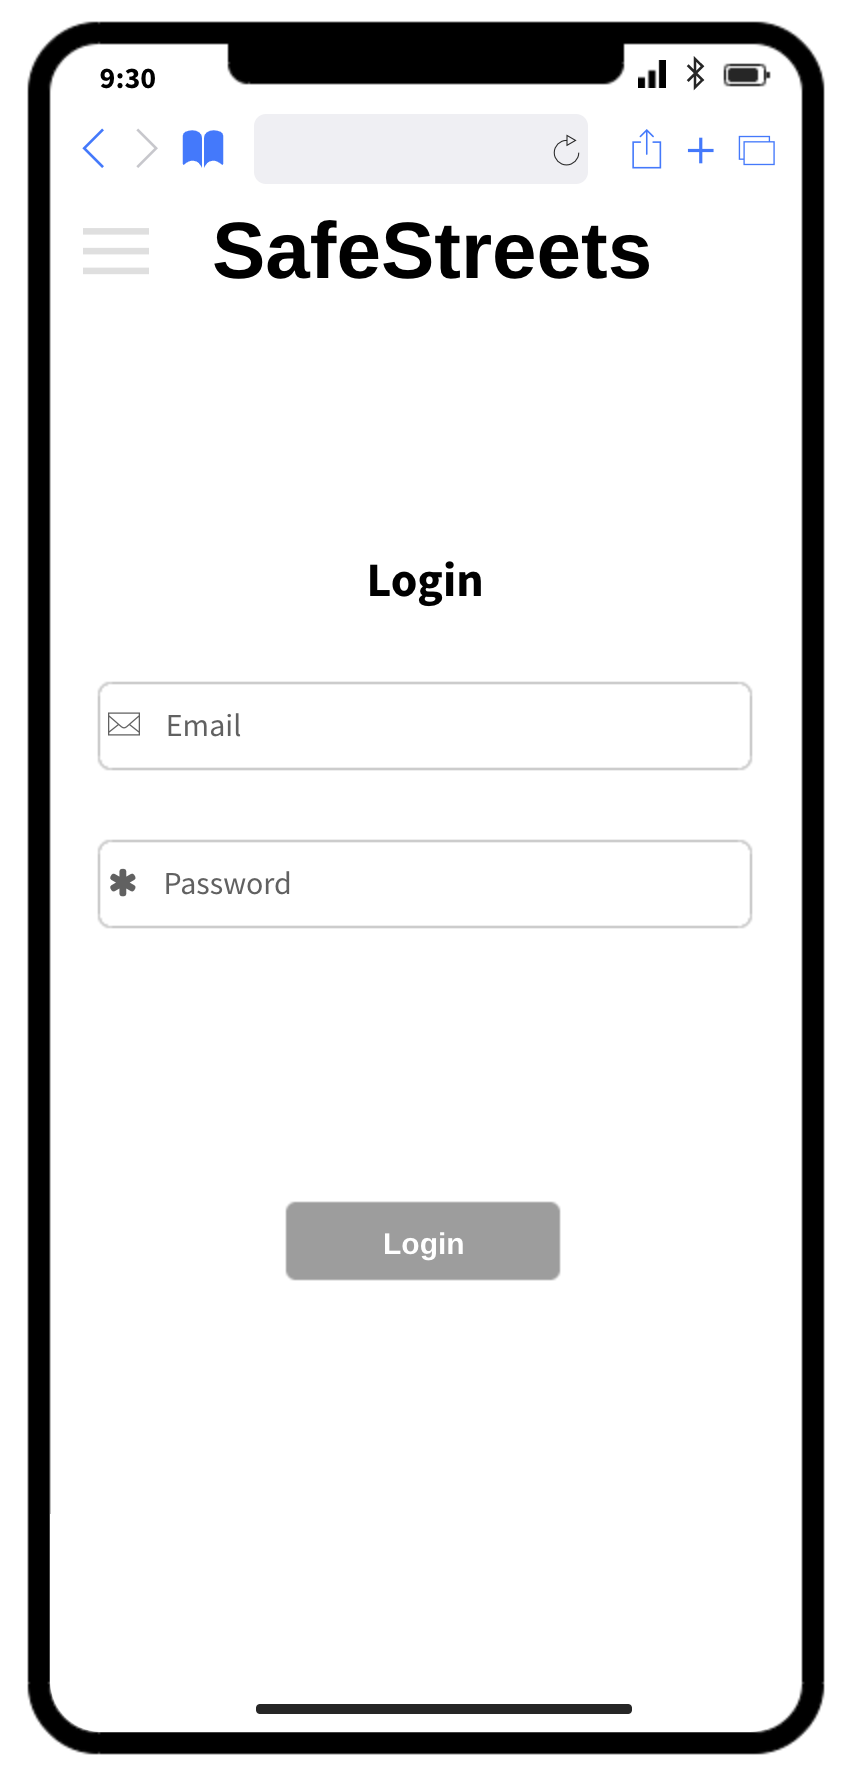
\includegraphics[width=\textwidth]{Images/login.png}
			\caption{Login form}
		\end{minipage}
		\hfill
		\begin{minipage}[b]{0.4\textwidth}
			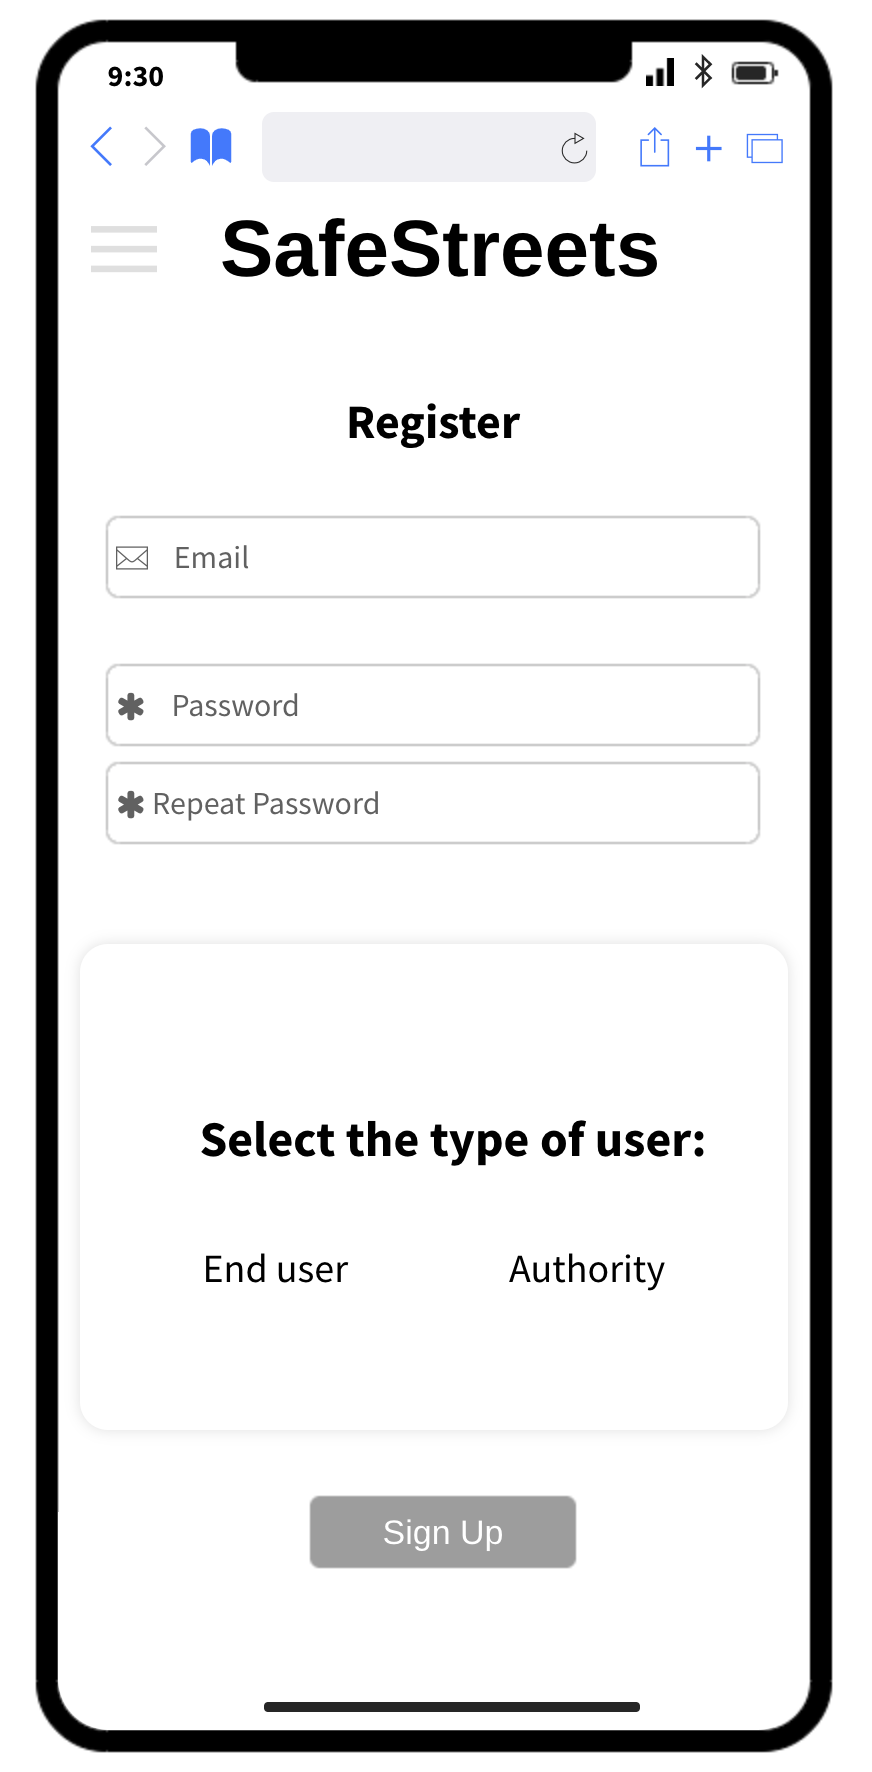
\includegraphics[width=\textwidth]{Images/registration.png}
			\caption{Registration form}
		\end{minipage}
	\end{figure}
	
		\begin{figure}[H]
		\centering
		\begin{minipage}[b]{0.40\textwidth}
			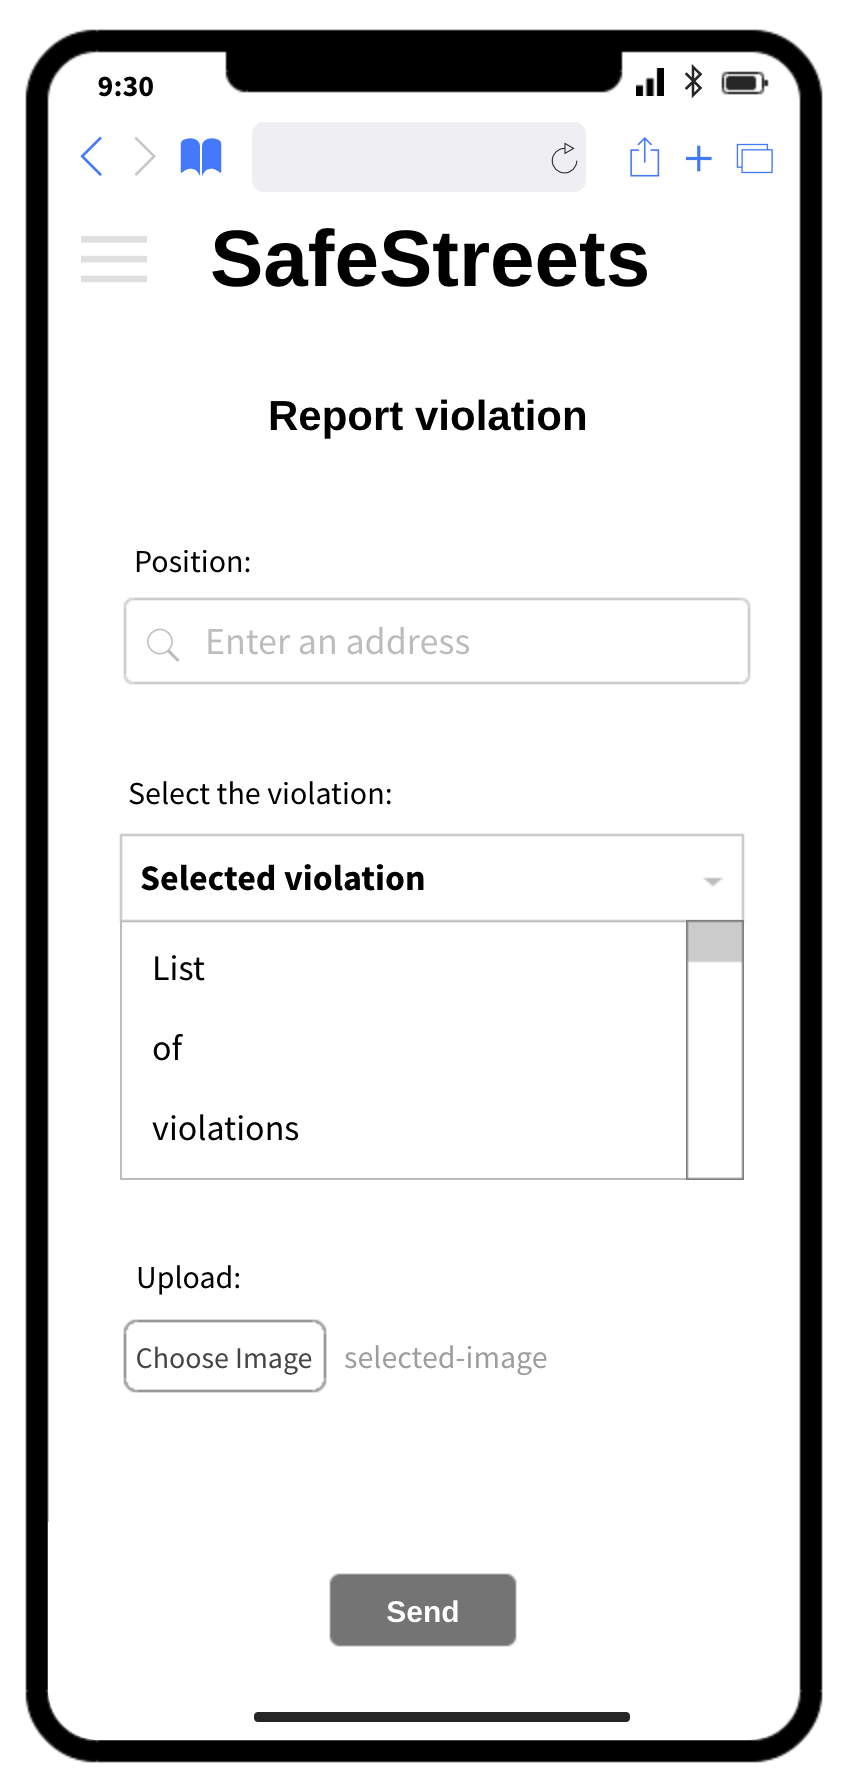
\includegraphics[width=\textwidth]{Images/report.png}
			\caption{User send violation report}
		\end{minipage}
		\hfill
		\begin{minipage}[b]{0.4\textwidth}
			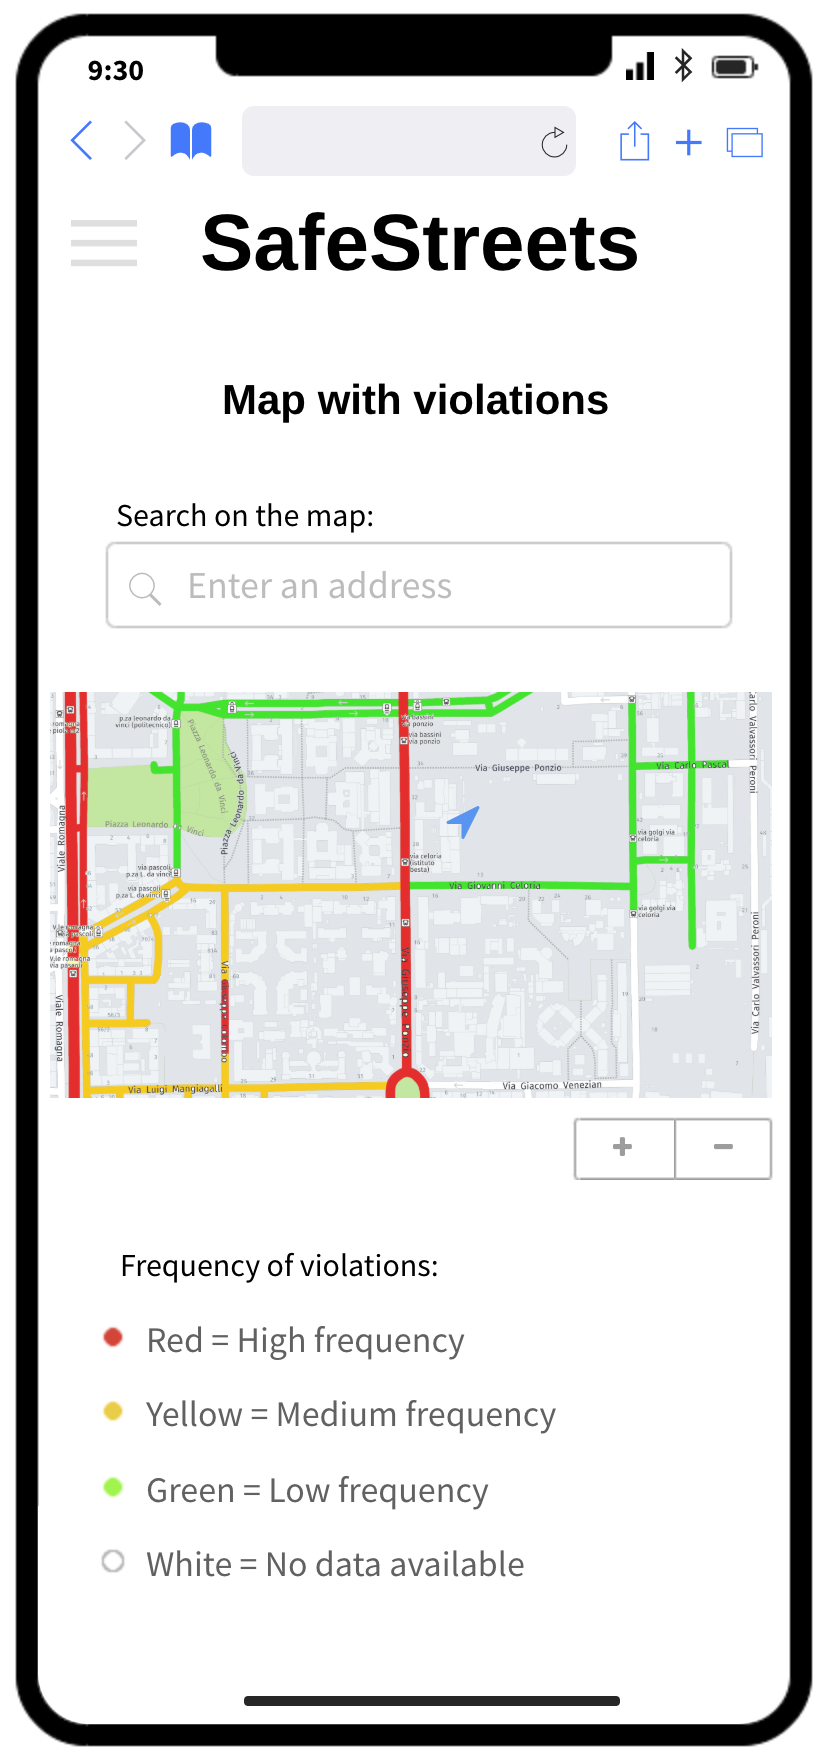
\includegraphics[width=\textwidth]{Images/violationsMap.png}
			\caption{Map showing violations}
		\end{minipage}
	\end{figure}

	\begin{figure}[H]
	\centering
	\begin{minipage}[b]{0.40\textwidth}
		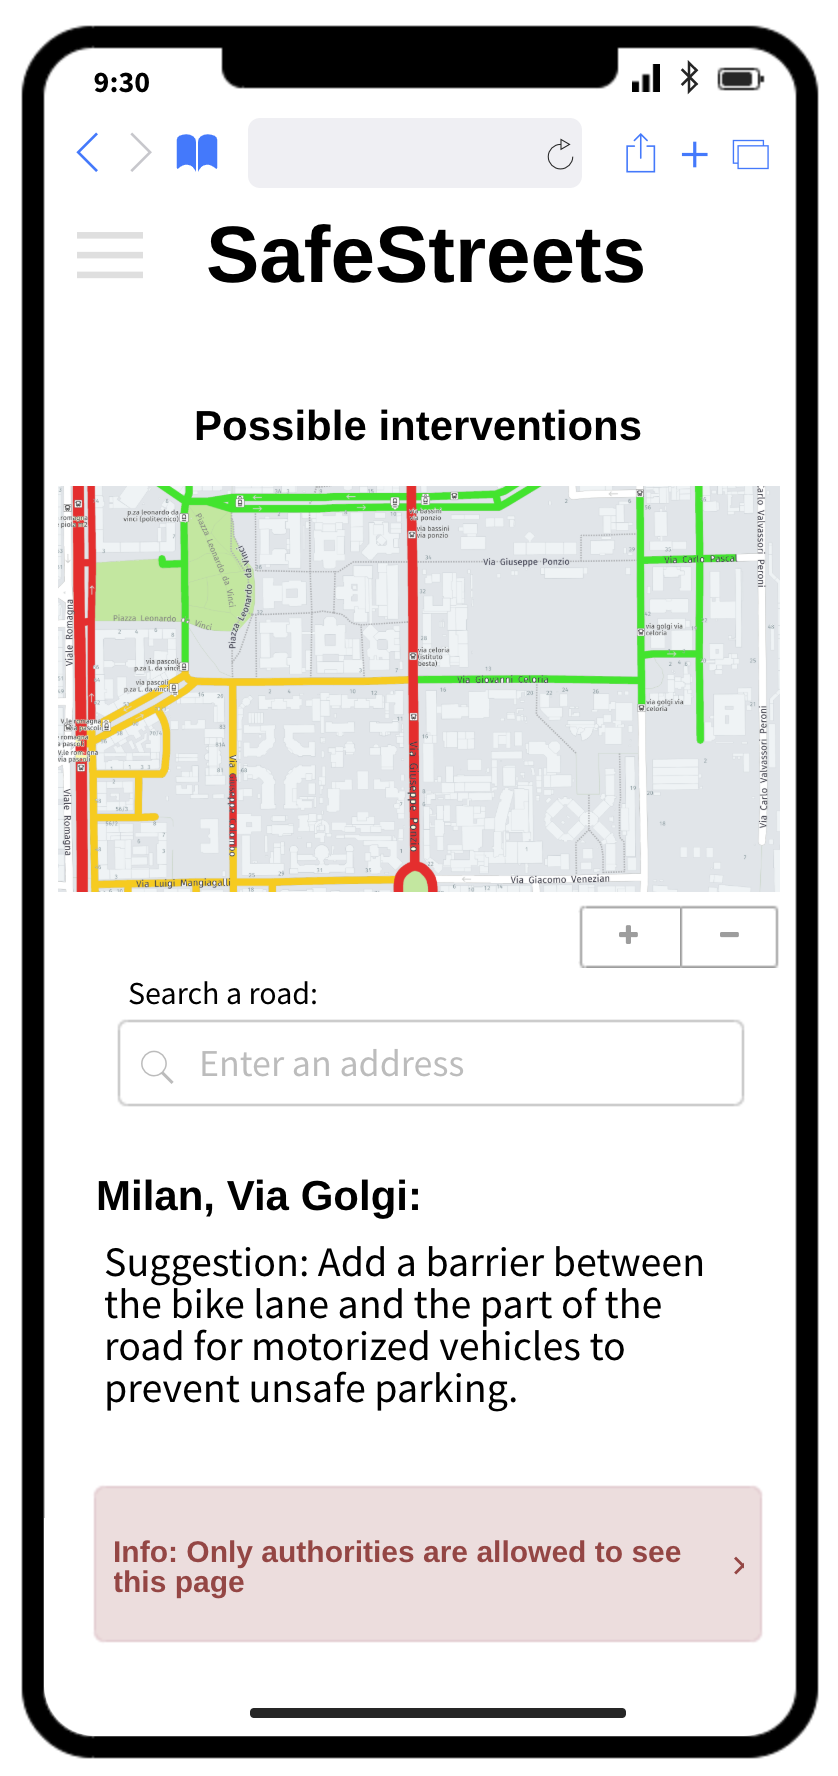
\includegraphics[width=\textwidth]{Images/interventions.png}
		\caption{Suggestion for possible interventions}
	\end{minipage}
	\hfill
	\begin{minipage}[b]{0.4\textwidth}
		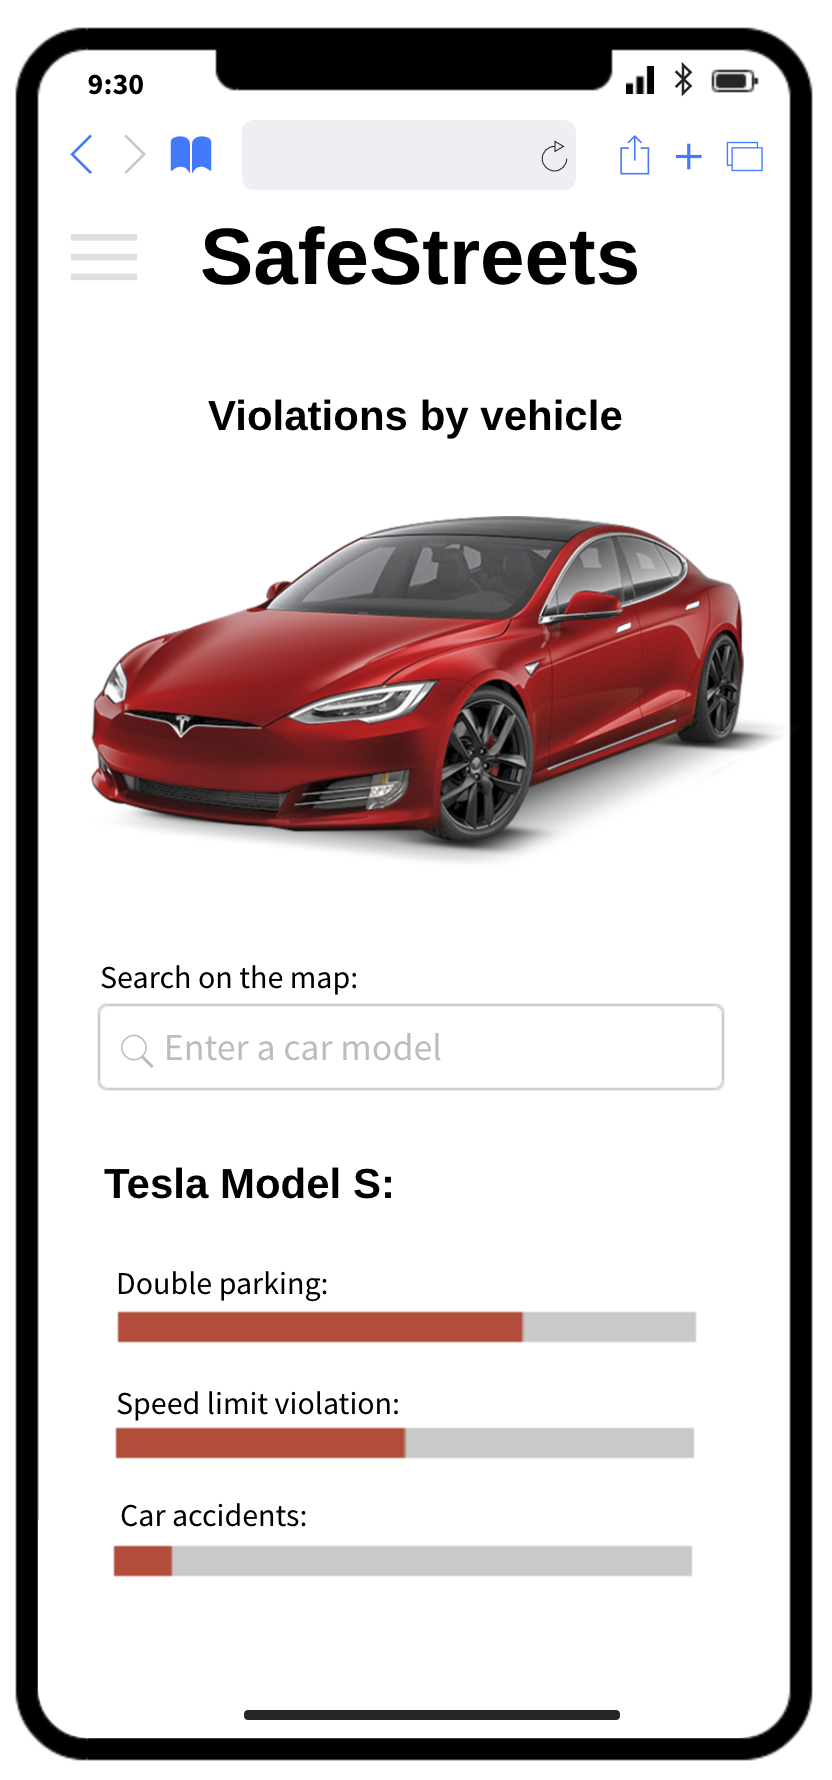
\includegraphics[width=\textwidth]{Images/vehicle.png}
		\caption{Violations by vehicle}
	\end{minipage}
\end{figure}

\subsubsection{Hardware interfaces}

\subsubsection{Software interfaces}
The system functionalities are provided without using third part application except for the CUU (Codice Univoco Ufficio) verification. This functions is made by an external web service provided by IndicePA. The code is required during the authorities registration to ensure their identity.
The external API are exposed only for authorities application and the implentation details will be shown in the design document.

\subsubsection{Communication interfaces}
Any communication functionality takes place via internet with HTTP protocol.
More in details, the protocol used is HTTPS, to allow protection and privacy.
This protocol will be used for both access to the web-application and REST communication.

\subsection{Design constraints}
\subsubsection{Standards compliance}
Part of the information collected by Safestreet (ex: license plate) are sensitive. For this reason the project is subject to the General Data Protection Regulation (GDPR). One of the technique used by the system to protect these important information is the creation of different type of user. For example normal account can only send information while authorities have a different account that is able to access to the data colleceted and generated.

\subsubsection{Hardware limitations}
The application is based on retrieving data from the photos sent by the user. Obviously the camera of the devices is a crucial aspect to consider during the design process. For this reason a minimun resolution of the sensor is required to install the application.The identification of this value will be done during design phase and will be written in the design document.
An other constraint is generated by the precision of the gps sensor of the device. Since the impact is smaller than the image resolution, the requirement is not so strict. 

\subsubsection{Any other constraint}
Safestreet works with violations and traffic tickets so it has to deal with law and regulation implications.
For this aspect see the specific domain assumption. 
Furthermore we have to consider the possible improper use of the platform. To prevent it Safestreet do some specific control on the images and is able to detect editing or repeated photos of the same violations. The implementation of this part will be done with some external algorithm and will be detailed in the design document.

\subsection{Functional requirements}
\subsubsection{Definition of use case diagram}
The use case diagrams provide a vision of the uses that can be done with the platform. They show the relationship between the actors and the use that every actor made with the software to reach the goals.

\subsubsection{Scenario 1}
Paul wants to sign up to SafeStreet platform. He has to insert his personal data (name, surname,place,mail etc.) and optionally also the car license plate. He will recieve a confirm mail and can use the platform.
\subsubsection{Scenario 2}
Bob is coming back to his car when he notice that someone has parked in double row and he can’t move. He log in into the safestreet app and he take a picture of the car to report it to the platform which analize the reporting and, in case it is true,it  could generate a traffic ticket and store the data to generate statistics.

\subsubsection{Scenario 3}
Luke is walking on the sidewalk when he see that a young guy is parking on a park reserved for disable.
Luke take a picture of the car and report it to the safestreet platform which analize the reporting and in case it could generate a traffic ticket and store the data to generate statistics.

\subsubsection{Scenario 4}
Mark has submitted a report to the safestreet platform, and he want to check if it has been accepted or declined.
He logs in into the app, he accesses to his reserved area and next to his report there is the status of message sent.

\subsubsection{Scenario 5}
Bill wants to check if someone has made a report on his car. He logs in into the platform and get the access to his profile where he can check if there is any traffic ticket for his car.

\subsubsection{Scenario 6}
The local authority wants to check which are the streets with more reports. They log in into the platform and access to their personal area where they can check the street status. They can set the color of the street based on the reports they recieve but also the platform automatically change the color of the streets based on the reports that recieve through the app.

 
\subsubsection{Scenario 7}
The local authority wants to check which are the vehicle with more reports. They log in into the platform and access to their personal area where they can check the cars that have the most reports assigned. They can set the color of the cars based on the reports they recieve but also the platform automatically change the color of the cars based on the reports that recieve through the app.

\subsubsection{Scenario 8}
The system recieves the photos from the users and have to check if they are true or fake. It runs an alghoritm that can detect if the photo is real or it has been modified. In the first case, the report will be stored and can be generate a traffic ticket. In the second case the report will be discarded.

\subsubsection{Scenario 9}
The local authority have to relase a traffic ticket in case of a user made an infringement. The platform auto-generate the trafic tickets when a report result real, and the local authority recieve a notify.

\subsection{Description of use case scenarios}
\subsubsection{Description scenario 1}


\begin{center}
	\begin{tabular}{ | l | p{6cm} | } 
		\hline
		ACTORS & Visitors  \\ 
		\hline
		GOALS & Sign up  \\ 
		\hline
		INPUT CONDITION & Personal data (name, surname, mail, telephone number, place where he lives, car license plate etc.)  \\ 
		\hline
		EVENTS FLOW & The user from the home page clicks on sign up. He inserts all of his information and if it is all correct he will recive an email of confirm.  \\ 
		\hline
		OUTPUT CONDITION & The user can now log in and use all the function that the user can do on the platform.  \\ 
		\hline
		EXCEPTIONS & Data incorrect, user already exists, mail already exists. All of this exceptions will be notified instantly to the user. \\ 
		\hline
	\end{tabular}
\end{center}

\subsubsection{Description scenario 2}

\begin{center}
	\begin{tabular}{ | l | p{6cm} | } 
		\hline
		ACTORS & User  \\ 
		\hline
		GOALS & Report a violation  \\ 
		\hline
		INPUT CONDITION & Type of violation (double row park), name of the street,  \\ 
		\hline
		EVENTS FLOW & The user take a picture of the car that has done the violation. The system use an algorithm to read the car license plate and then store all the informations once it is established that the photo isn't fake.  \\ 
		\hline
		OUTPUT CONDITION & The violation has been stored with all the data, it will be generated a traffic ticket, and the local authority can decide to highlight who has made the violation or the street. \\ 
		\hline
		EXCEPTIONS & Data incorrect or fake photo. The report will be discarded and no traffic ticket will be generated.  \\ 
		\hline
	\end{tabular}
\end{center}

\subsubsection{Description scenario 3}

\begin{center}
	\begin{tabular}{ | l | p{6cm} | } 
		\hline
		ACTORS & User  \\ 
		\hline
		GOALS & Report a violation  \\ 
		\hline
		INPUT CONDITION & Type of violation (wrong park), name of the street,  \\ 
		\hline
		EVENTS FLOW & The user take a picture of the car that has done the violation. The system use an algorithm to read the car license plate and then store all the informations once it is established that the photo isn't fake.  \\ 
		\hline
		OUTPUT CONDITION & The violation has been stored with all the data, it will be generated a traffic ticket, and the local authority can decide to highlight who has made the violation or the street. \\ 
		\hline
		EXCEPTIONS & Data incorrect or fake photo. The report will be discarded and no traffic ticket will be generated.  \\ 
		\hline
	\end{tabular}
\end{center}

\subsubsection{Description scenario 4}

\begin{center}
	\begin{tabular}{ | l | p{6cm} | } 
		\hline
		ACTORS & User  \\ 
		\hline
		GOALS & Check report status  \\ 
		\hline
		INPUT CONDITION & User credentials  \\ 
		\hline
		EVENTS FLOW & The user log in into the platform. He accesses to his personal area and he can check the status of his report \\ 
		\hline
		OUTPUT CONDITION & Report status \\ 
		\hline
		EXCEPTIONS & The user hasn't made any report. The system show a messagge that the list of the reports is empty.  \\ 
		\hline
	\end{tabular}
\end{center}

\subsubsection{Description scenario 5}

\begin{center}
	\begin{tabular}{ | l | p{6cm} | } 
		\hline
		ACTORS & User  \\ 
		\hline
		GOALS & Check his profile  \\ 
		\hline
		INPUT CONDITION & User credentials  \\ 
		\hline
		EVENTS FLOW & The user log in into the platform. He accesses to his personal area and he can check if his car has recieved some report \\ 
		\hline
		OUTPUT CONDITION & Car status \\ 
		\hline
		EXCEPTIONS & The user hasn't a car or hasn't recived any report. The system show a messagge that there isn't any report.  \\ 
		\hline
	\end{tabular}
\end{center}

\subsubsection{Description scenario 6}

\begin{center}
	\begin{tabular}{ | l | p{6cm} | } 
		\hline
		ACTORS & Local authority  \\ 
		\hline
		GOALS & Check streets status  \\ 
		\hline
		INPUT CONDITION & Local authority credentials  \\ 
		\hline
		EVENTS FLOW & The authority log in into the platform. He accesses to his personal area and he can check the streets status \\ 
		\hline
		OUTPUT CONDITION & Different colors for the streets based on their status and possibly changes to the color of some streets \\ 
		\hline
		EXCEPTIONS & none \\ 
		\hline
	\end{tabular}
\end{center}

\subsubsection{Description scenario 7}

\begin{center}
	\begin{tabular}{ | l | p{6cm} | } 
		\hline
		ACTORS & Local authority  \\ 
		\hline
		GOALS & Check cars status  \\ 
		\hline
		INPUT CONDITION & Local authority credentials  \\ 
		\hline
		EVENTS FLOW & The authority log in into the platform. He accesses to his personal area and he can check the cars status based on reports \\ 
		\hline
		OUTPUT CONDITION & Different colors for the cars based on how many reports they recived and possibly changes to the color of some cars \\ 
		\hline
		EXCEPTIONS & none \\ 
		\hline
	\end{tabular}
\end{center}

\subsubsection{Description scenario 8}

\begin{center}
	\begin{tabular}{ | l | p{6cm} | } 
		\hline
		ACTORS & SafeStreets  \\ 
		\hline
		GOALS & Check the reliability of the photo  \\ 
		\hline
		INPUT CONDITION & Photo that has been taken by a user.  \\ 
		\hline
		EVENTS FLOW & The system recives from the user a photo of a possibile violation. It runs an algorithm that can establish if it is real or fake. \\ 
		\hline
		OUTPUT CONDITION & The photo is real of fake. \\ 
		\hline
		EXCEPTIONS & none \\ 
		\hline
	\end{tabular}
\end{center}

\subsubsection{Description scenario 9}

\begin{center}
	\begin{tabular}{ | l | p{6cm} | } 
		\hline
		ACTORS & SafeStreets  \\ 
		\hline
		GOALS & Generate trafic tickets  \\ 
		\hline
		INPUT CONDITION & Report  \\ 
		\hline
		EVENTS FLOW & If the report is real than it could be generated the trafic ticket based on the type of violation the user has committed. \\ 
		\hline
		OUTPUT CONDITION & Trafic ticket \\ 
		\hline
		EXCEPTIONS & The report is fake, nothing is generated. \\ 
		\hline
	\end{tabular}
\end{center}

\subsection{Software system attributes}
\subsubsection{Reliability}
The system has to ensure reliability, to this scope we have decided to keep a backup server, that operate every 24h.
The system also use an algorithm to ensure that the reports of violations that the system recive, are real and not modified or fake.
\subsubsection{Availability}
The platform has to be available every day, especially in the rush hours because are the hours where there are more traffic and it could be useful to be active in that time. SafeStreets must have 99\% (3.65 days/year downtime).
\subsubsection{Security}
The data have to be crypted, to grant the privacy (ex.user's position, car license plate etc.). It could be useful to use HTTPS protocol to transmit data from user to SafeStreets.
Every account must have a strong password with the combination of upper-case, lower-case letters, numbers and punctuation.
\subsubsection{Maintainability}
The system is programmed to be compatible with other platform, like the system of the local authority.
There could be maintenance interventions, when it's possible there will be in the hours with the less use of the platform.
There will be released updates, both for application and system.
\subsubsection{Portability}
The entire system is portable, every user (citizen or local authority) can access to their profile, see data, statisthics and make reports of violation from their mobile or their tablet, not especially from PCs.
\subsection{Mapping on requirements}
\begin{center}
	\begin{tabular}{ | l | p{2cm} | p{2cm}| p{2cm}|} 
		\hline
		 RawID & GoalID & ReqID & Use Case ID \\
		\hline
		1&G1&RE.1&Scenario 2/3\\
		\hline
		2&G2.1&RE.2&\\
		\hline
		3&G2&RE.3&\\
		\hline
		4&G3.1&RE.4&Scenario 6\\
		\hline
		5&G3&RE.5&\\
		\hline
		6&G4&RE.6&\\
		\hline
		7&G5&RE.7&Scenario 8\\
		\hline
		8&G2&RE.8&Scenario 9\\
		\hline
	\end{tabular}
\end{center}


 

%------------------------------------------------------------------------------------------------------------------------------------------------
\clearpage
{\color{Blue}{\section{Formal Analysis Using Alloy}}}
\label{sect:alloy}
During the draft of the alloy, we omitted the aspects regarding the chain of custody because, as mentioned in Security description (3.7.3), these controls are made before storing information in the system, thus the other portions of the application are able to ignore it.

For this reason there is no constraint in Alloy that checks the fact that the report and the image can only exist if the information are genuine.
\newpage

\subsection{Alloy code}
\begin{figure}[!htbp]
	\centering
	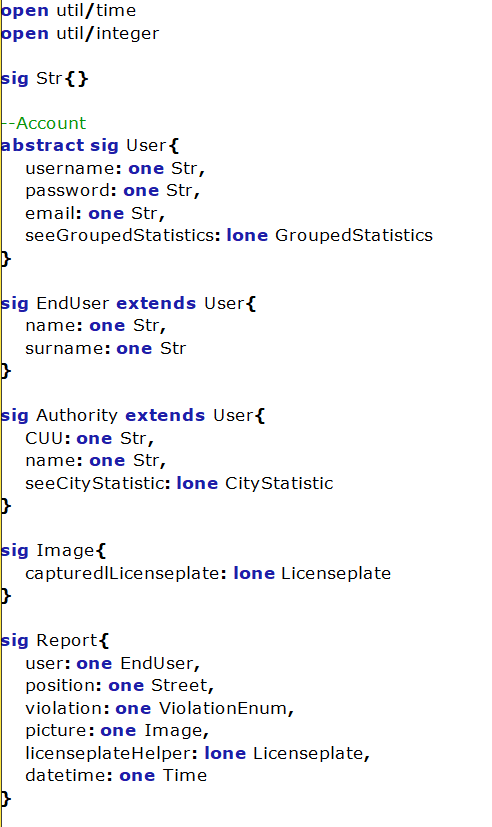
\includegraphics[width=0.9\linewidth, height=0.8 \textheight]{Images/Alloy/codealloy1}
	\caption{Signature 1}
	\label{Signature 1}
\end{figure}

\begin{figure}[h]
	\centering
	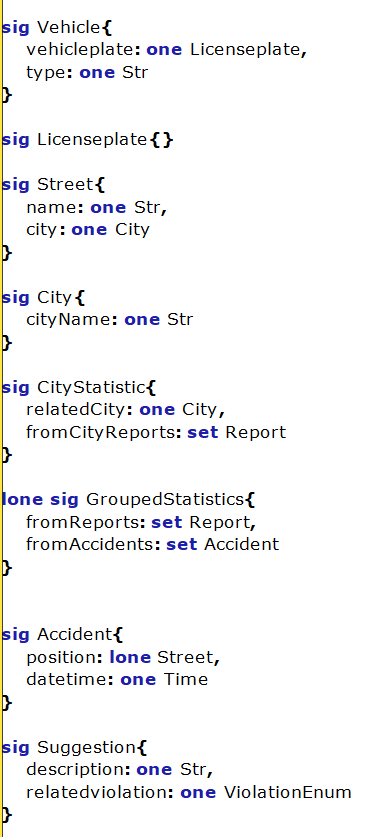
\includegraphics[width=0.5\linewidth, height=0.65\textheight]{Images/Alloy/codealloy2}
	\caption{Signature 2}
	\label{Signature 2}
\end{figure}

\begin{figure}[h]
	\centering
	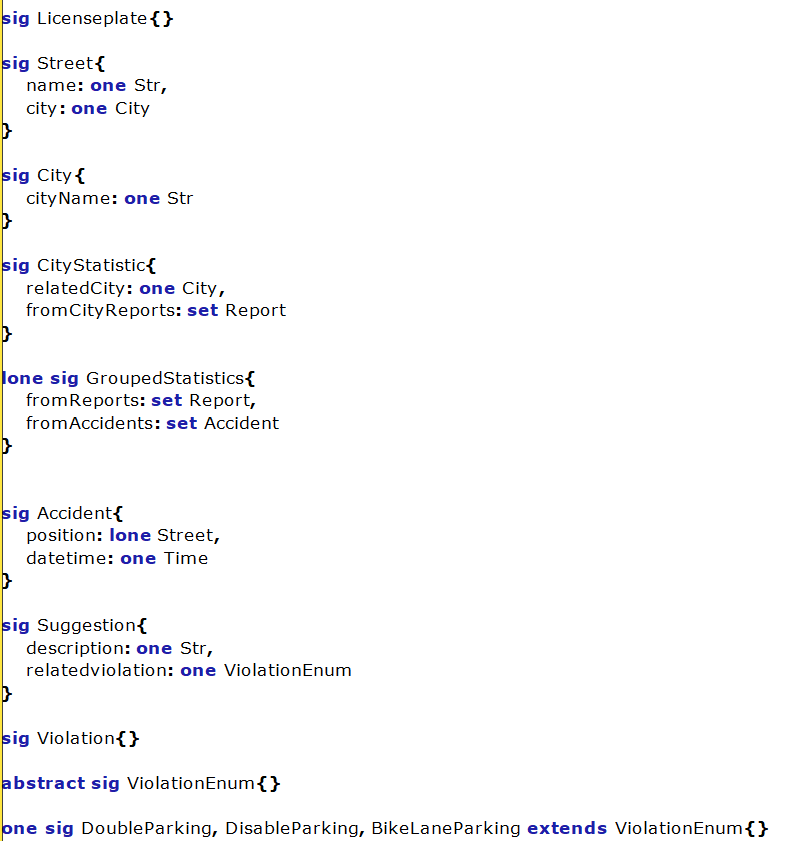
\includegraphics[width=0.9\linewidth, height=0.7\textheight]{Images/Alloy/codealloy3}
	\caption{Signature 3}
	\label{Signature 3}
\end{figure}

\begin{figure}[h]
	\centering
	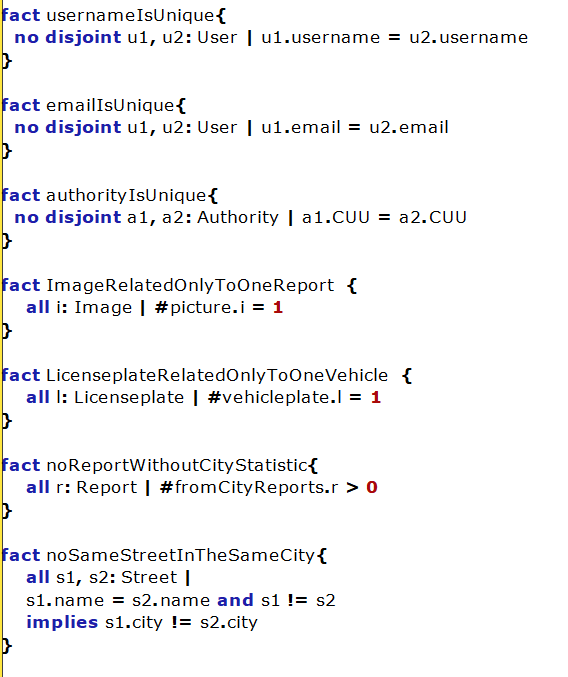
\includegraphics[width=0.9\linewidth, height=0.8\textheight]{Images/Alloy/codealloy4}
	\caption{Pred and Facts 1}
	\label{Pred and Facts 1}
\end{figure}

\begin{figure}[h]
	\centering
	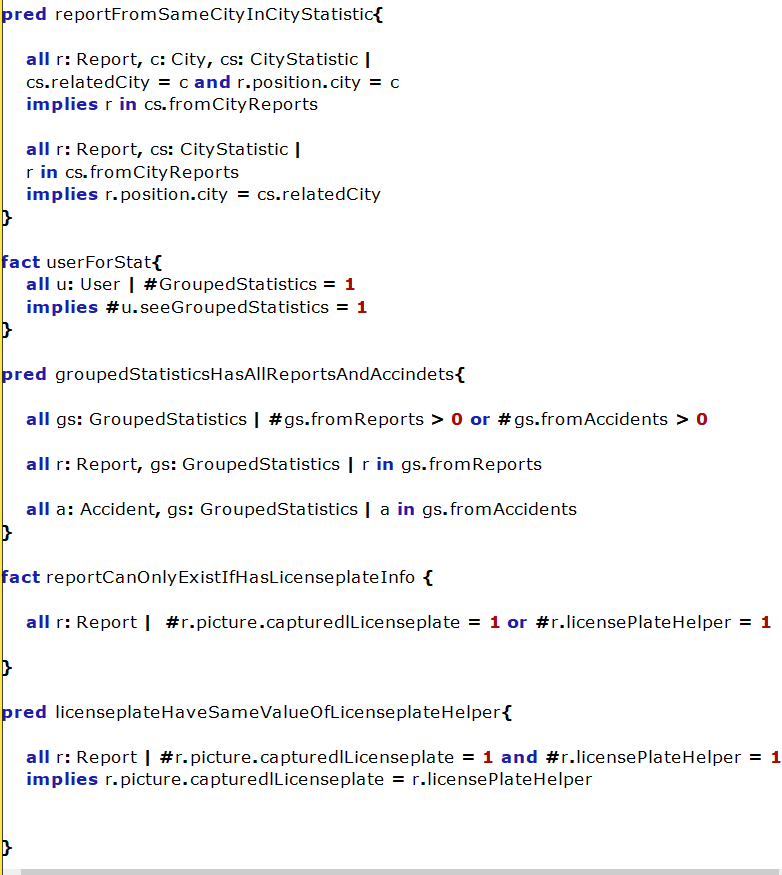
\includegraphics[width=0.9\linewidth, height=0.8\textheight]{Images/Alloy/codealloy5}
	\caption{Pred and Facts 2}
	\label{Pred and Facts 2}
\end{figure}

\begin{figure}[h]
	\centering
	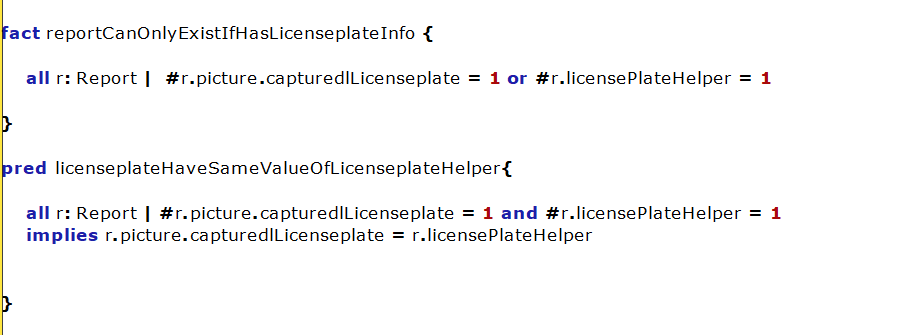
\includegraphics[width=0.9\linewidth, height=0.3\textheight]{Images/Alloy/codealloy6}
	\caption{Pred and Facts 3}
	\label{Pred and Facts 3}
\end{figure}

\begin{figure}[h]
	\centering
	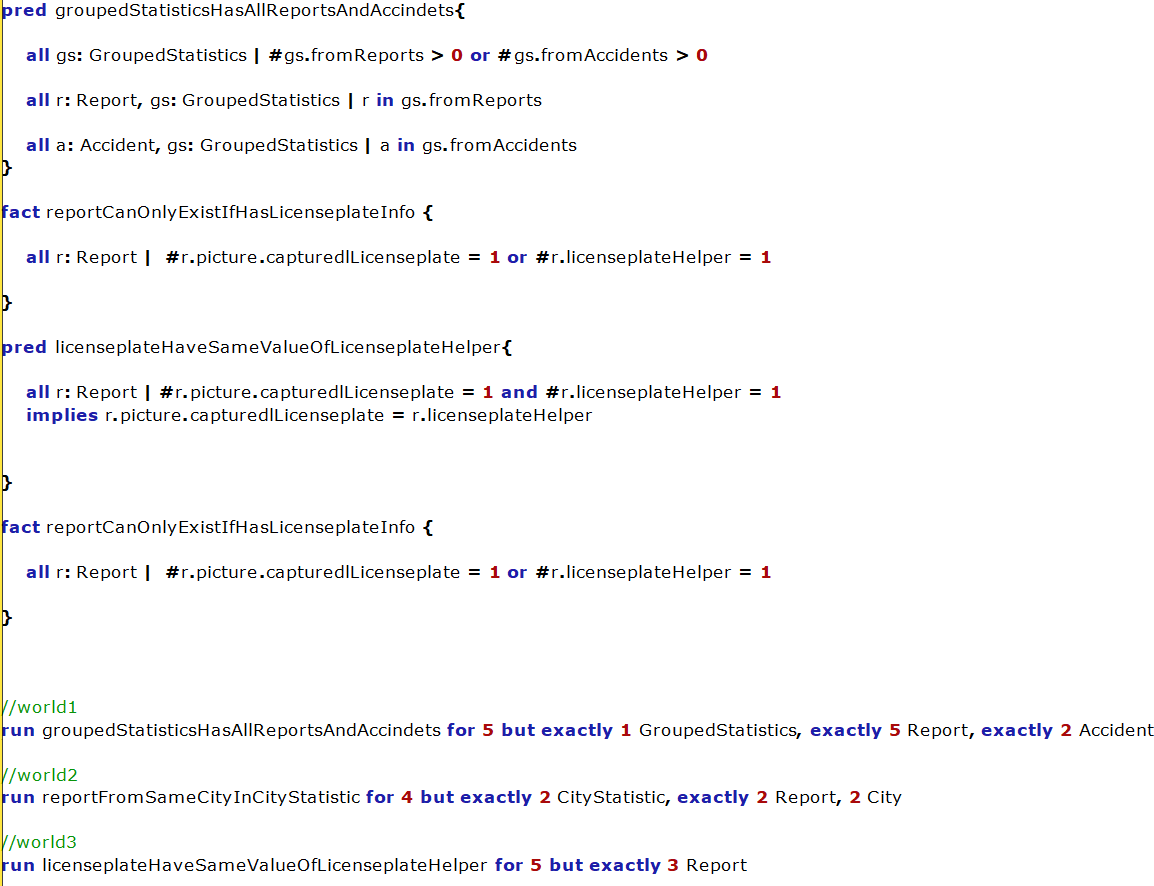
\includegraphics[width=0.95\linewidth, height=0.86\textheight]{Images/Alloy/codealloy7}
	\caption{Pred, Facts and World}
	\label{Pred and Facts and World}
\end{figure}
\FloatBarrier
\subsection{Predicates testing}
\subsubsection{World 1}
Predicate about the aggregation of data coming from reports with the traffic information.

This predicate describes the constraint that the signature that represent statistics can only exist if and only if there is at least one report or accident.
Furthermore all reports and all accidents must be related to statistics.
\begin{figure}[h]
	\centering
	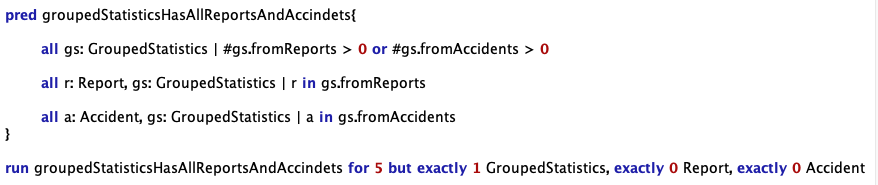
\includegraphics[width=0.9\linewidth, height=0.15\textheight]{Images/Alloy/test-world11}
	\caption{Pred 1}
	\label{Pred 1}
\end{figure}
\FloatBarrier
To show that the predicate works as expected, we have run the predicate with with inconsistent number of sig entities: exactly of  0 reports and 0 accidents but 1 GroupedStatistic
\begin{figure}[h]
	\centering
	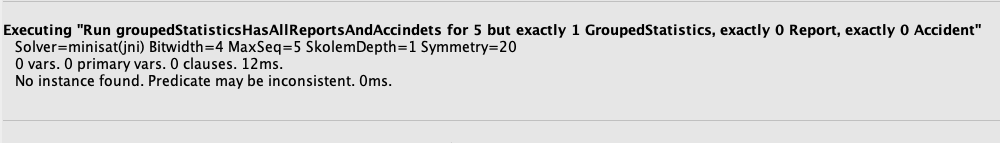
\includegraphics[width=0.9\linewidth, height=0.12\textheight]{Images/Alloy/test-world12}
	\caption{Result pred 1}
	\label{Result pred 1}
\end{figure}
\FloatBarrier
\newpage
The following represented world is generated from the following run: run groupedStatisticsHasAllReportsAndAccindets for 5 but exactly 1 GroupedStatistics, exactly 5 Report, exactly 2 Accident
\begin{figure}[h]
	\centering
	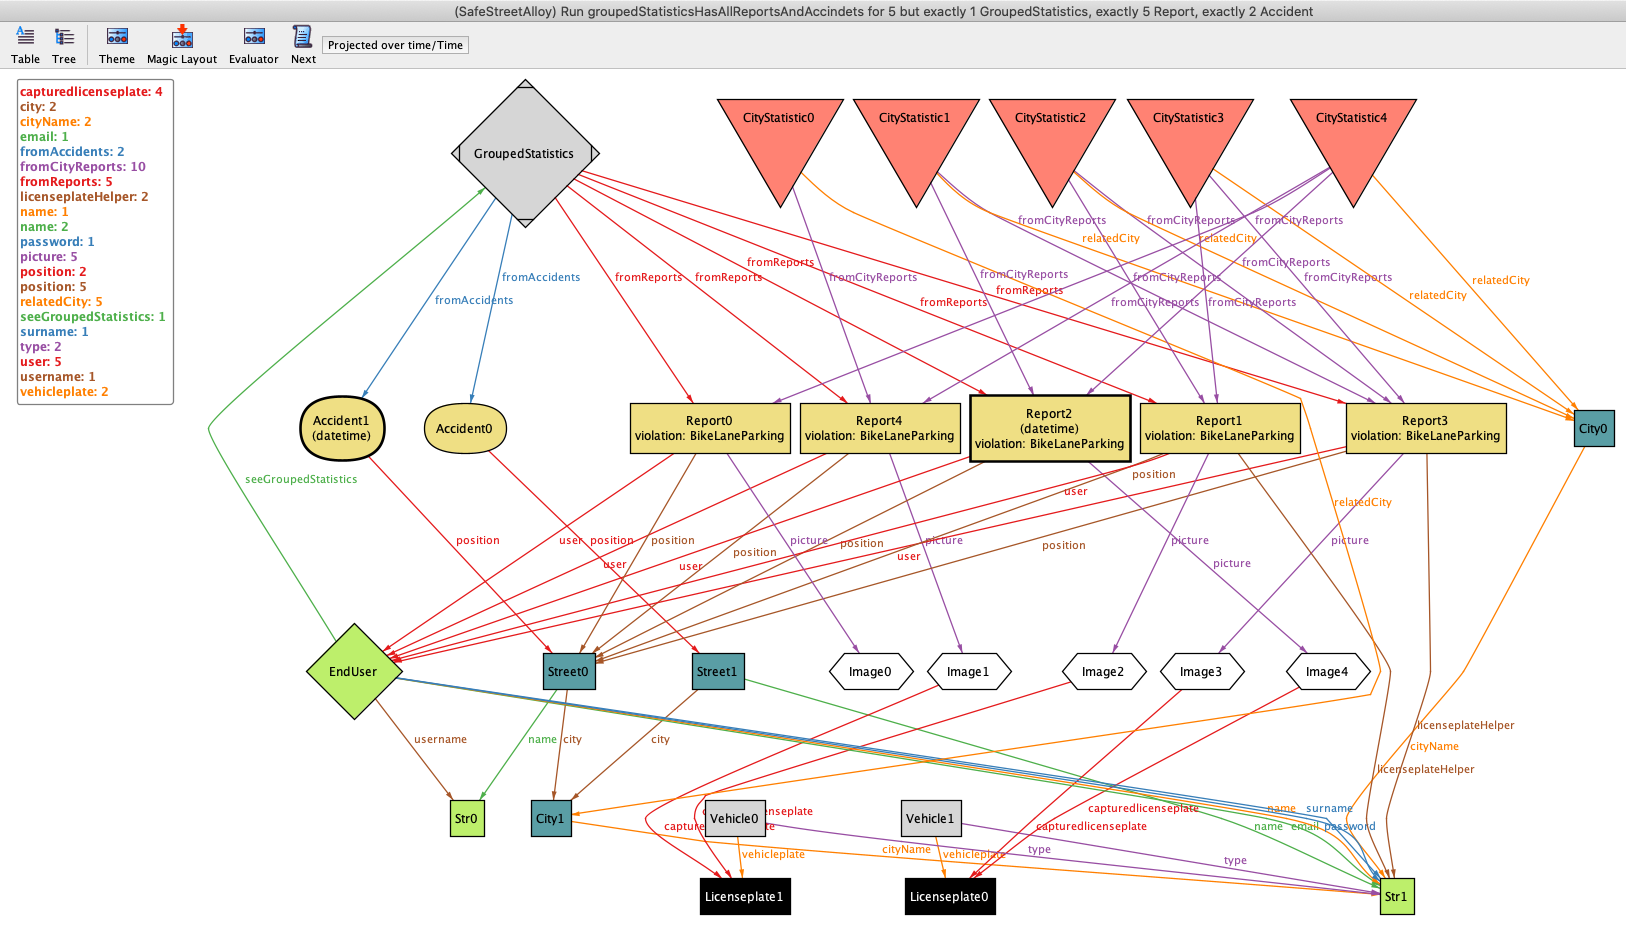
\includegraphics[width=0.9\linewidth, height=0.5\textheight]{Images/Alloy/world1}
	\caption{World 1 generated by pred 1}
	\label{World1 }
\end{figure}
\FloatBarrier
\newpage
\subsubsection{World 2}
Consistency between city and statistics.

This predicate describes the constraint that the signature that represent statistics specific about a city and all reports about all streets of the city must be related.
\begin{figure}[h]
	\centering
	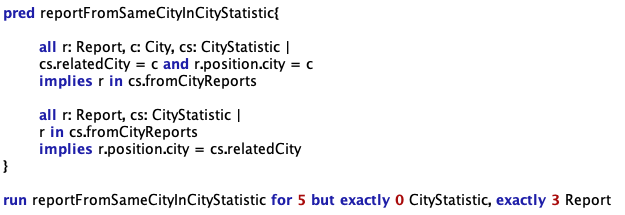
\includegraphics[width=0.9\linewidth, height=0.15\textheight]{Images/Alloy/test-world21}
	\caption{Pred 2}
	\label{Pred 2}
\end{figure}
\FloatBarrier
To show that the predicate works as expected, we have run the predicate with with inconsistent number of sig entities: exactly 0 CityStatistic, exactly 3 Report.
\begin{figure}[h]
	\centering
	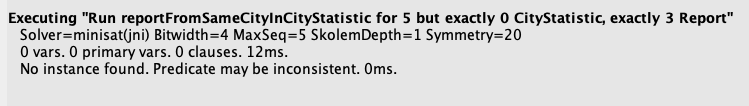
\includegraphics[width=0.9\linewidth, height=0.11\textheight]{Images/Alloy/test-world22}
	\caption{Result pred 2}
	\label{Result pred 2}
\end{figure}
\FloatBarrier
\newpage
The following represented world is generated from the following run: run reportFromSameCityInCityStatistic for 4 but exactly 2 CityStatistic, exactly 2 Report, 2 City
\begin{figure}[h]
	\centering
	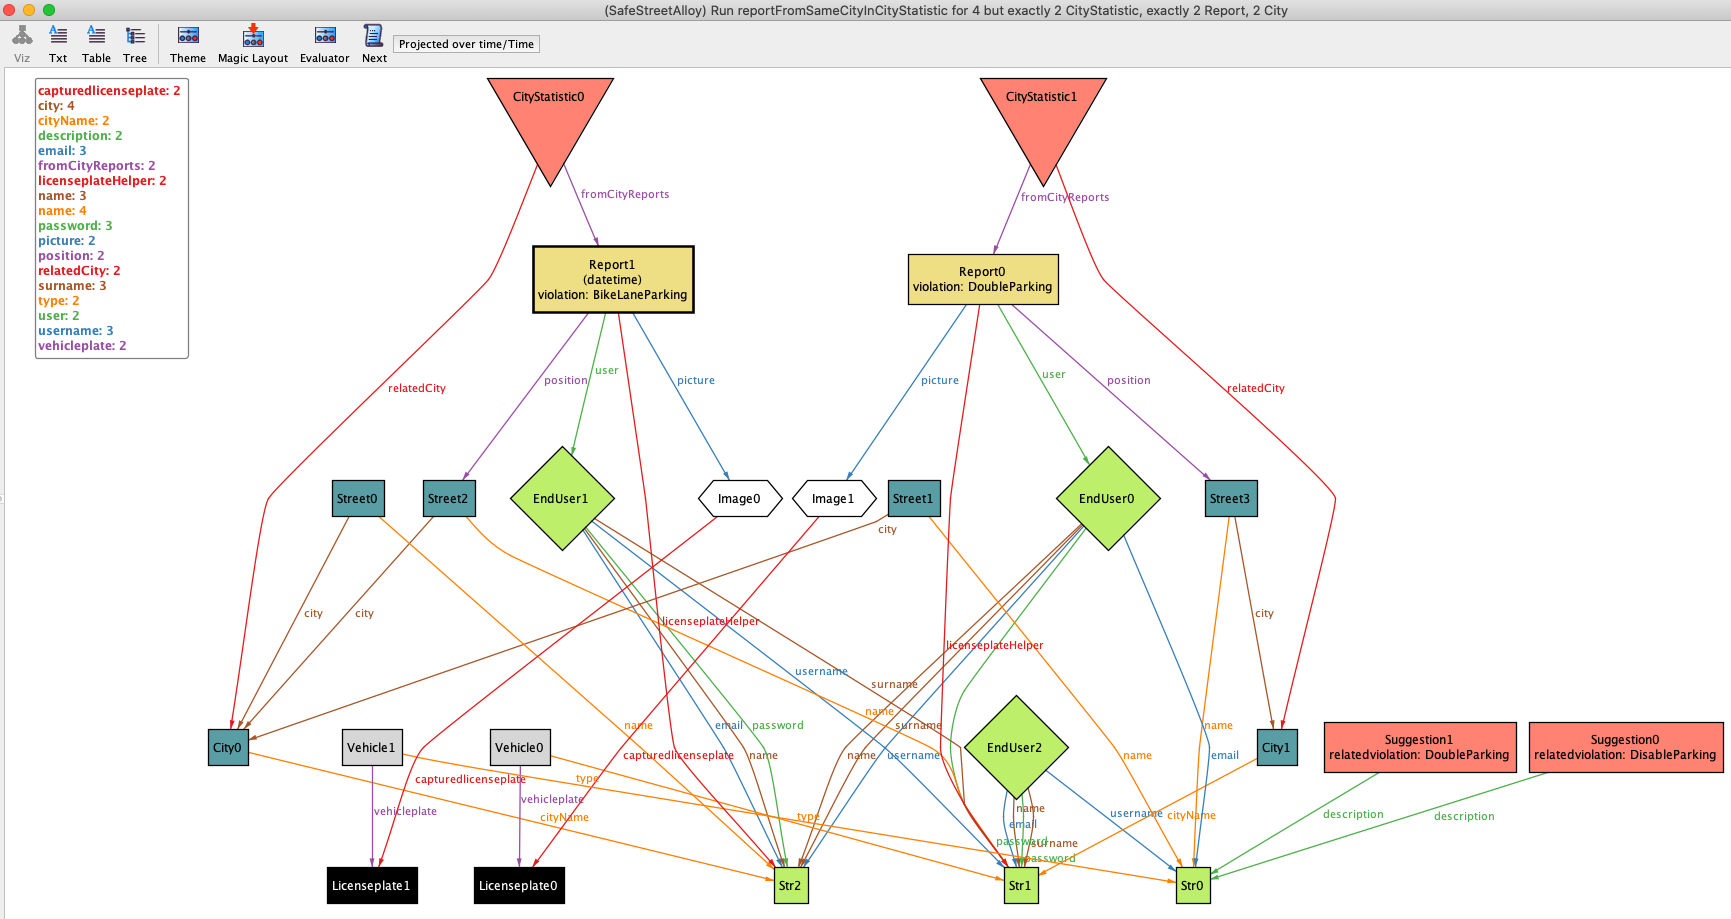
\includegraphics[width=1\linewidth, height=0.47\textheight]{Images/Alloy/world2}
	\caption{World 2}
	\label{World2}
\end{figure}
\FloatBarrier
\newpage
\subsubsection{World 3}
Predicate that test if the licenseplate retrieve from SafeStreets is the same suggested by the user.
\begin{figure}[h]
	\centering
	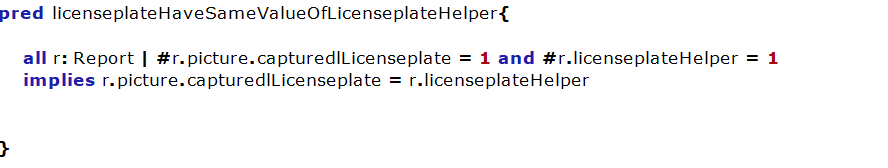
\includegraphics[width=0.9\linewidth, height=0.15\textheight]{Images/Alloy/predworld31}
	\caption{Predicate 3}
	\label{Pred 3}
\end{figure}

\begin{figure}[h]
	\centering
	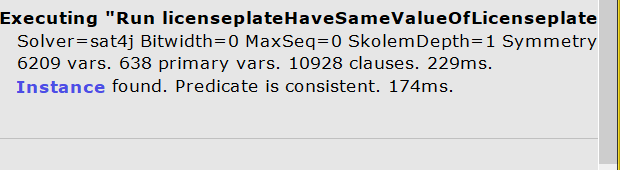
\includegraphics[width=0.8\linewidth, height=0.11\textheight]{Images/Alloy/predworld32}
	\caption{Result pred 3}
	\label{Result pred 3}
\end{figure}
\FloatBarrier
\newpage
The following represented world is generated from the following run: run licenseplateHaveSameValueOfLicenseplateHelper for 5 but exactly 3 Report
\begin{figure}[h]
	\centering
	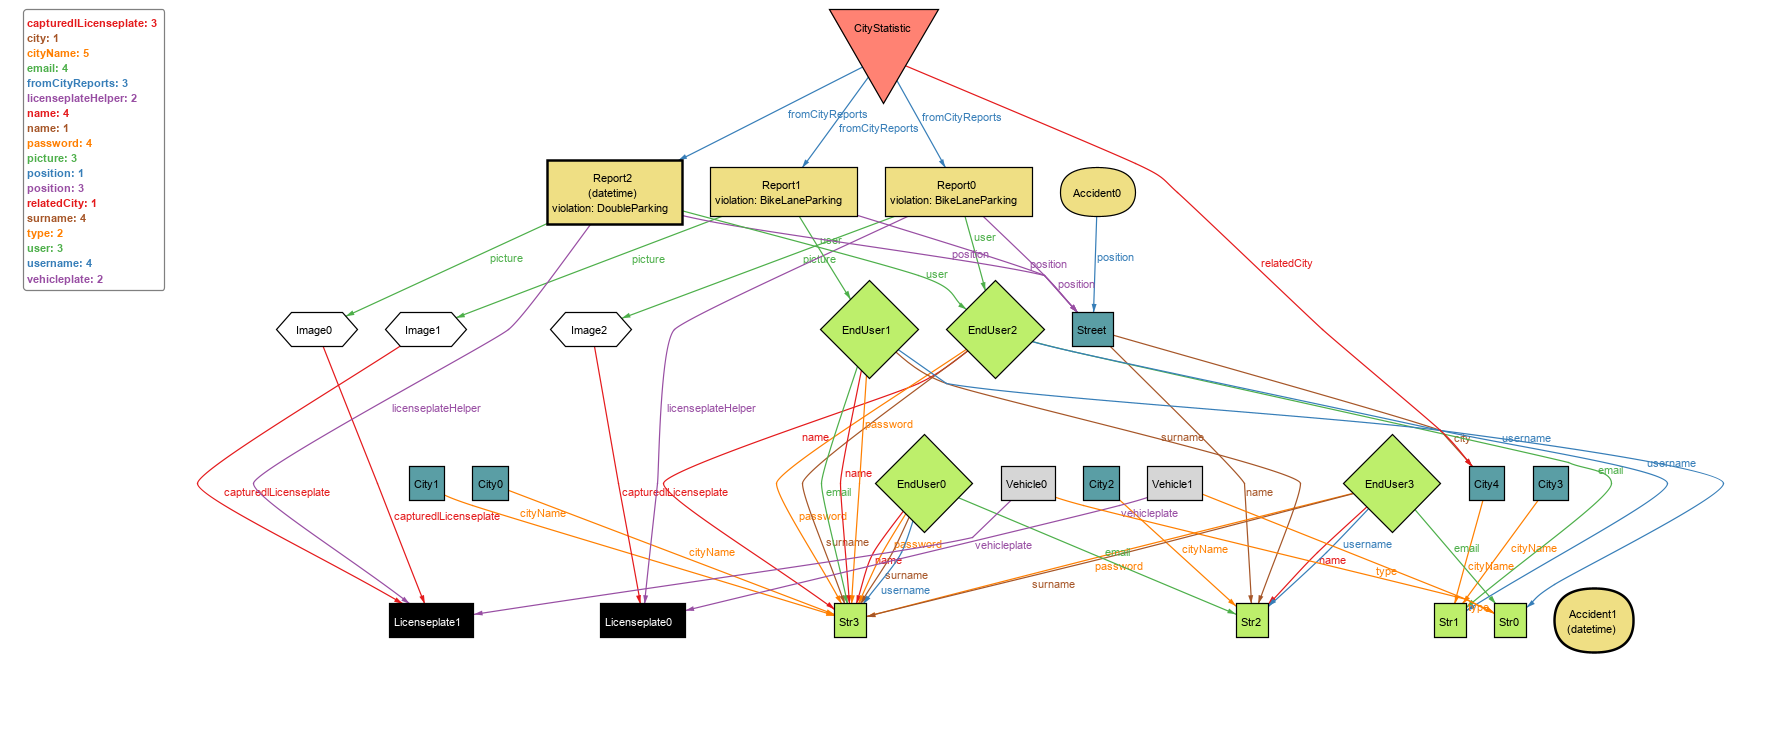
\includegraphics[width=1.1\linewidth, height=0.55\textheight]{Images/Alloy/world3alloy}
	\caption{World 3}
	\label{World3}
\end{figure}


%------------------------------------------------------------------------------------------------------------------------------------------------
\clearpage
{\color{Blue}{\section{Effort Spent}}}
\label{sect:effort}
\hfill
\subsubsection{Ivan Cavadini}
\hfill
\begin{center}
	\begin{tabular}{ | l | p{6cm} | } 
		\hline
		TASK & TIME \\ 
		\hline
		Purpose & 2h  \\ 
		\hline
		Scope & 2h  \\ 
		\hline
		Definitions, Acronyms, Abbreviations & 1h \\ 
		\hline
		Overview & 3h \\ 
		\hline
		Runtime view & 10h \\ 
		\hline
		Requirements traceability & 1h \\ 
		\hline
		Various & 5h  \\ 
		\hline
		TOTAL & 24h \\ 
		\hline
	\end{tabular}
\end{center}
\hfill
\newpage
\subsubsection{Nicolò Molinari}
\hfill
\begin{center}
	\begin{tabular}{ | l | p{6cm} | } 
		\hline
		TASK & TIME \\ 
		\hline
		Component view & 12h  \\ 
		\hline
		Deployment view & 3h  \\ 
		\hline
		Revision history & 0.5h \\ 
		\hline
		Component interfaces & 3h \\ 
		\hline
		Implementation, integration and test & 3h \\ 
		\hline
		Database structure & 1h   \\ 
		\hline
		Various & 4h \\ 
		\hline
		TOTAL & 26.5h \\ 
		\hline
	\end{tabular}
\end{center}
\hfill
\newpage
\subsubsection{Luigi Pederzani}
\hfill
\begin{center}
	\begin{tabular}{ | l | p{6cm} | } 
		\hline
		TASK & TIME \\ 
		\hline
		Revision history & 2h  \\ 
		\hline
		Selected architectural styles and pattern & 8h  \\ 
		\hline
		Other design decisions  & 4h \\ 
		\hline
		User characteristics & 4h \\ 
		\hline
		User Interface design & 5h \\ 
		\hline
		Various & 1.5h  \\ 
		\hline
		TOTAL & 24.5h \\ 
		\hline
	\end{tabular}
\end{center}


\newpage
\subsection{Versions}
\hfill
\hfill
\begin{center}
	\begin{tabular}{ | l | p{6cm} | } 
		\hline
		VERSIONS & DESCRIPTION  \\ 
		\hline
		1.0 & Introduction creation   \\ 
		\hline
		1.1 & Introduction review  \\ 
		\hline
		2.0 & Overview draft \\ 
		\hline
		2.1 & Database structure \\ 
		\hline
		2.2 & Added class diagram \\ 
		\hline
		2.3 & Added component view   \\ 
		\hline
		2.4 & Added runtime view (sequence diagrams)  \\ 
		\hline
		2.5 & Creation of component interfaces \\ 
		\hline
		3.0 & Writing out Selected architectural styles and patterns \\ 
		\hline
		3.1 & Added description of Other design decisions \\ 
		\hline
		4.0 & Creation of UI mocks  \\ 
		\hline
		4.1 & Added screens routing \\ 
		\hline
		5.0 & First draft of Requirements traceability \\ 
		\hline
		5.1 & Requirements traceability correction \\ 
		\hline
		6.0 & Writing out Implementation \\ 
		\hline
		6.1 & Writing out Test \\ 
		\hline
		7.0 & Document review \\ 
		\hline
		7.1 & Final version \\ 
		\hline
	\end{tabular}
\end{center}

\subsection{Used Tools}

\begin{itemize}
	\item TeXstudio 2.12.14
	\item Magic Draw 19.0
	\item MockFlow
	\item Dropbox Paper
\end{itemize}



%------------------------------------------------------------------------------------------------------------------------------------------------
\clearpage
\addcontentsline{toc}{section}{References}
\bibliographystyle{plain}
\bibliography{main}
%------------------------------------------------------------------------------------------------------------------------------------------------




\end{document}
